\chapter{Enabling Applications in Creative Writing}
\label{chap:creativity}
One application where NLG has considerable potential is in the development of tools for creative writing. AI-assisted creative writing is an attractive testbed NLG systems because ideation tools are already part of writers' arsenal, and mistakes like hallucinating false facts are less problematic in fiction than in domains like automatic news summarization, where faithfulness to the real world is crucial. In addition, writers have been grappling with the concept of sentient, human-like machines for at least as long as computer scientists have.

In this chapter, I describe work I have done toward bridging the gap between what most language models do by default (predict a continuation for a prompt) and the operations writers actually would want.
First, I will describe efforts to capture longer-term coherence by building a language model that operates over sentences rather than other sub-words.
Second, I will show how existing neural networks can be modified to support fill-in-the-blank style tasks in addition to the more common paradigm of continuation.
Filling in the blank is a common control that is requested by writers.
Third, I will present a recipe for performing sentence style transfer into arbitrary styles--such as rewriting text to be more Shakespearean, metaphorical, or meladramatic--without any exemplars of the task or task-specific model training.

To test out how these and other NLG-based tools can be used in practice, we built Wordcraft, a word processor augmented with a variety of ``smart'' writing controls and suggestion tools.
I will end by describing the features of Wordcraft and the results of a user study conducted with the tool.

\section{Motivation}
Artificial intelligence systems which can write stories have been a goal of researchers since the early days of computing.
However, much of the early work in this area was focused on building systems which could produce an entire story from scratch given an initial set of constraints.

Rather than focusing on developing NLG systems which produce entire stories, my research in this area focuses on enabling better human-AI collaboration.


\section{Models for Infilling Text}
\label{section:fitb}

\subsection{Motivation}
% Main contributions
% First to propose using the same model for both fill-in-the-blank and continuation.
% First to compare against strategies which do not require any fine-tuning.
% First to show how models trained on general data transfer to out-of-domain data.

Natural language generation systems are increasingly being incorporated into applications where a human writer and an AI jointly collaborate to construct text.
Wordcraft, The AI-assited text processor I describe in Section \ref{section:wordcraft} is one such application.
Another is Storium, where players of a writing game, have the option to accept suggestions from a natural langueg generatin system \citep{akoury2020storium}.
There are also more practical domain such as email composition assistance and code synthesis \citep{buschek2021impact,wu2018smart,austin2021program}.
Many of these applications are limited to generating text at the end of what has been written so far.
This is because
both historical language models (LMs) and state-of-the-art neural LMs
are typically designed to produce text by repeatedly predicting the next word in a sequence given the previous words.
However, there is a need for more powerful interactive tools which enable writers to solicit insertions at any chosen position within the existing text, a task variously referred to as fill in the blank (\FitB), infilling, or the Cloze task \citep{taylor1953cloze}.
For example, a creative writer might want a tool which can insert a description of a place or character, and a programmer might want a system that can fill in a method in the middle of their code.

\begin{figure}[t]
    \centering
    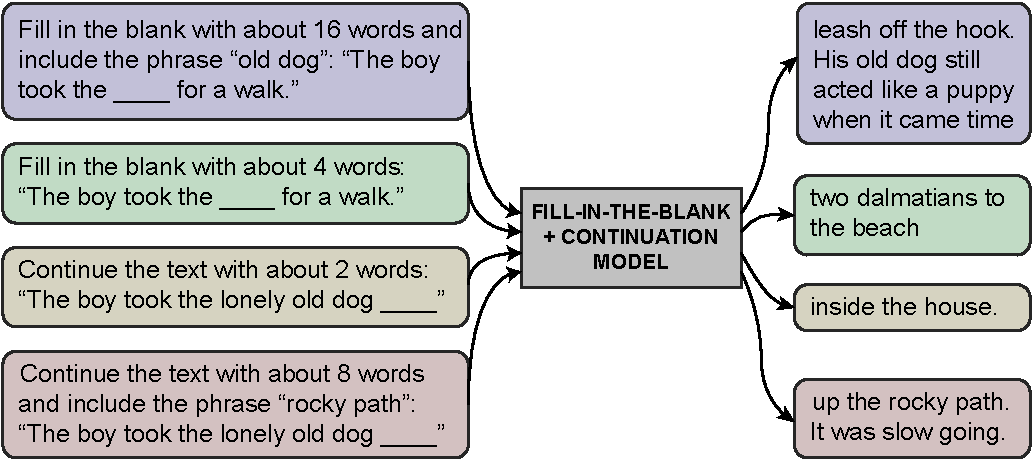
\includegraphics[width=0.48\textwidth]{figures/leading_figure.pdf}
    \caption{A single model that can handle a variety of related writing tasks is more efficient than separate models per task.}
    \label{fig:leading_figure}
    \vspace{-1em}
\end{figure}

Most prior work tackling \FitB{} consider it a separate task from continuation, one to be specifically optimized for, for example training a custom model from scratch \citep{ippolito2019unsupervised,zhu2019text,mori2020finding}, finetuning a model trained originally for continuation \citep{donahue2020enabling}, or using a combination of pre-trained models \citep{huang2020inset}.
Having separate trained models for \FitB{} and for continuation is inefficient for downstream applications where maintaining multiple neural networks can b e prohibitive.

Any model that can do \FitB{} can be made to do continuation simply by placing the blank at the end of the input.
Thus, in this section, we describe how models trained on \FitB{} can be employed effectively for both infilling and continuation operations.
We show how T5 \citep{raffel2019exploring}, one of the most popular pre-trained models, can reasonably handle both tasks, as it was pre-trained with a \FitB-like objective.
Finetuning T5 further improves its ability and also allows for the incorporation of controllability of generation length and word choice.


\begin{table}[t]
  \centering
  \small
  \caption{Examples of the finetuning objectives. ``8" is the approximate length in words of the target sequence. During finetuning, about 25\% of training examples took each of these formats.}
    \begin{tabular}{p{0.12\textwidth}p{0.57\textwidth}p{0.20\textwidth}}
    \midrule
    Example Type & Input & Target \\
    \midrule
     \cFITB{} no goal & fill: I love avocados. I ate a sandwich covered in them. {\textbf \_8\_} I talked to my doctor about it later. It turned out I was allergic to avocados. & After I ate it, my mouth was itchy and tingly. \\
    \midrule
     \cFITB{}  with goal & fill: I love avocados. I ate a sandwich covered in them.  {\textbf \_8\_} I talked to my doctor about it later. It turned out I was allergic to avocados.  {\textbf Goal: mouth was itchy} & After I ate it, my mouth was itchy and tingly. \\
    \midrule
     \cFITB{} no goal& fill: I love avocados. I ate a sandwich covered in them. After I ate it, my mouth was itchy and tingly. I talked to my doctor about it later.  {\textbf \_8\_}  & It turned out I was allergic to avocados. \\
    \midrule
     \cFITE{} with goal & fill: I love avocados. I ate a sandwich covered in them. After I ate it, my mouth was itchy and tingly. I talked to my doctor about it later.  {\textbf \_8\_}   {\textbf Goal: allergic to} & It turned out I was allergic to avocados. \\
    \midrule
    \end{tabular}
   \vspace{-0.6em}
  \label{tab:task_examples}
  \vspace{-1em}
\end{table}%

\subsection{Supporting \FitB{} and Continuation}
\label{section:fitb_fite_methods}
We define filling in the blank as the task of predicting text to replace a single missing span, usually demarcated with a special token, in an input text passage. (Some prior work considers inputs with multiple blanks, but inserting text at one position at a time better matches the kinds of edits humans do.)
We define continuation in the traditional language modeling sense--predicting the next token in a sequence given only the previous tokens.
\citet{donahue2020enabling} discuss how language modeling is a special case of infilling, and they use this as justification to finetune a continuation-based language model to do infilling.
However, we argue that if continuation is a subtask of infilling, it makes more sense to go in the opposite direction: prioritize a model which can do infilling and check that it achieves satisfactory performance at continuation.

T5 is a model pre-trained with a ``span corruption'' objective very similar to \FitB; the model is asked to reconstruct the missing text after random sub-sequences of the input are replaced with special identifiers.
Thus, a pre-trained T5 model can be used without any further training to do both continuation and infilling by appropriately choosing text to mask out.
The encoder-decoder architecture of T5 is also more conducive to \FitB{} than decoder-only architectures like GPT-2 \citep{radford2019language} which are typically used for continuation-based language models.
This is because the attention mechanism in encoder-decoder architectures allows the context on the left side of the blank to attend to the context on the right, while decoder-only architectures only support masked attention (each token can only attend to the positions to its left).

Even though T5's pre-training objective was a form of \FitB, finetuning is still advantageous.
For one, our definition of \FitB{} only includes a single masked out substring, not multiple, so finetuning improves alignment with the goal task.
% Furthermore,
Finetuning also allows us to incorporate additional conditioning signals not supported by the pre-trained T5, such as being able to specify the desired length of the generated text or specify words that ought to be included in the blank, a task we refer to as ``goal conditioning."
Length control, which comes by default in a traditional language model
%since one can simply sample
by simply sampling more or fewer
tokens, is particularly necessary for \FitB, where the end of the generation must fit seamlessly with the text to its right.

The biggest language models available today were largely trained in the continuation rather than the \FitB{} paradigm \citep{gpt3,gpt-neo}.
Since our primary goal is to have a single model for both tasks, we also address the question: if a continuation-trained model is big enough, can it handle \FitB{} without the need for finetuning?
Few-shot learning with large language models, as popularized by \citet{gpt3}, has had success on many tasks in NLP.
We try out this approach for \FitB{} by designing a few-shot prompt containing several demonstrations of the \FitB{} task, formulated in a similar ``infilling by language modelling" style as \citet{donahue2020enabling}.

\subsection{Experimental Setup}
For all primary experiments, we use the 800M parameter v1.1 `large' model.
We also show soome addditional results comparing against the 3B parameter `XL' T5 model.
To finetune T5 for \FitB, we construct training examples from documents by first partitioning the document text into a left context, gap, and right context.
The input sequence is then the left and right contexts concatenated with textual representations of the additional conditioning signals.
The target sequence is the true text for the blank.
This formulation easily supports continuation, as the blank can be deliberately placed at the end (i.e., providing no right context).
Documents are drawn from C4, the same dataset T5 was pre-trained on.
Documents are split into word sequences, and these are then randomly truncated to be between 256-512 words long.
A substring of between 1 and 64 words is selected to be blanked out.
For half of the training examples the blank is randomly selected, and for the other half it is always placed at the end.
To support length conditioning, we follow \citet{roberts2020exploring} and include a bucketed version of the target length as part of the blank.
To support goal conditioning, for half the examples, a random substring of up to half the words of the target is appended to the end of the input.
Examples are shown in Table \ref{tab:task_examples}.

We compare T5 against a state-of-the-art 137B parameter decoder-only language model (\LLM{}) trained explicitly for continuation and used successfully for few-shot learning in other domains \citep{austin2021program,reif2021recipe}.
%This model is used (1) as a standard continuation model, passing in only the left context of an example as the prompt; and (2) in a few-shot learning paradigm.
This model is used (1) as a standard continuation model, prompting with only the left context of an example; and (2) in a few-shot learning paradigm.

We evaluate continuation and \FitB{} on C4 as well as two story writing datasets, as creative writing assistant applications are one of the key areas we expect to benefit from multi-task models \citep{wordcraft}.
Reddit Writing Prompts (\textsc{Rwp}) is a corpus of stories from the `r/WritingPrompts' sub-Reddit \citep{fan2018hierarchical}, and we construct validation sets \rwpFITB{} and \rwpFITE{} using the same method described in the previous section.
C4 and \textsc{Rwp} validation sets are capped to 5,000 examples.
% We also include a third validation set \rwpFITS, where gaps are randomly chosen but always exactly one sentence long.
ROC Stories (\textsc{Roc}) is a crowd-sourced dataset of five-sentence commonsense stories \citep{mostafazadeh2016corpus}.
For ROC Stories, the 2018 validation set is used to construct \rocFITB, where the middle sentence of each story is blanked out, and \rocFITE, where the last sentence is blanked out.
Unless otherwise noted, all evaluation is done without goal conditioning and uses random sampling with top-$k$=50 as the decoding strategy.
Example generations for all evaluation sets can be found at \url{https://bit.ly/2U0Ixxa}.

\begin{table}[t]
\small
\centering
    \caption{Perplexity of evaluation sets according to \LLM{} when the blank has been filled with approaches involving no fine-tuning (top), finetuned approaches (middle), and the groundtruth (bottom).
    Lower values indicate that the text was considered more fluent by the \LLM{}.
    \label{tab:generative_ppl_results}
    }
    \begin{tabular}{l|rrr}
    \toprule
    %  & \cFITB & \rocFITB & \rwpFITB & \rwpFITB-Sent \\
    & \textsc{C4Fill} & \textsc{RwpFill} & \textsc{RocFill} \\ % & \textsc{RwpFill} \\
    & \textsc{Blank} & \textsc{Middle} & \textsc{Blank} \\ % & \textsc{Blank}-Sent \\
    % \cline{2-5}
    \midrule
    {Few-shot \LLM} & 14.14 & 19.48 & 18.21 \\ % & 16.36 \\
    % {Pre-trained T5 XL} & 10.27 & 13.94 & 21.75 \\ % & TODO \\
    {Pre-trained T5} & 10.38 & 14.08 & 22.62 \\ % & 10.49 \\
    \midrule
    % {\FITBFITE{} XL} & 11.49 & 15.05 & 24.87 \\ % & 10.33 \\
    {Finetuned T5} & 10.33 & 14.08 & 20.47 \\ % & 10.37 \\
    {\citet{donahue2020enabling}} & N/A & N/A & 23.28 \\ % & N/A \\
    
    \midrule
    {Groundtruth} & 9.41 & 12.99 & 16.90 \\

    \bottomrule
    \end{tabular}
\end{table}

\begin{table}[t]
    \caption{Perplexity of continuation-based evaluation sets when a continuation has been generated using approaches with no finetuning (top) and two settings of finetuning T5 (middle).}
    \label{tab:generative_ppl_continuation_results}
    \centering
    \small
    \begin{tabular}{l|rrr}
    \toprule
    %  & \cFITB & \rocFITB & \rwpFITB & \rwpFITB-Sent \\
    & \textsc{C4Fill} & \textsc{RwpFill} & \textsc{RocFill} \\
    & \textsc{End} & \textsc{End} & \textsc{End}  \\
    % \cline{2-5}
    \midrule
    % {\LLM} & TODO  & TODO & TODO \\
    {Pre-trained T5}  & 10.09 & 13.51 & 21.71 \\
    \midrule
    % {\FITBFITE{} XL}  & 10.77 & 14.66 & 22.66 \\
    {T5 \FITBFITE{}} & 10.04 & 13.74 & 19.60 \\
    {T5 \textsc{Lm-Adaption}} & 10.06  & 13.71 & 19.68 \\
    \midrule
    {Groundtruth} & 9.41 & 12.99 & 16.90 \\
    \bottomrule
    \end{tabular}
\end{table}

\begin{figure}[t]
    \centering
    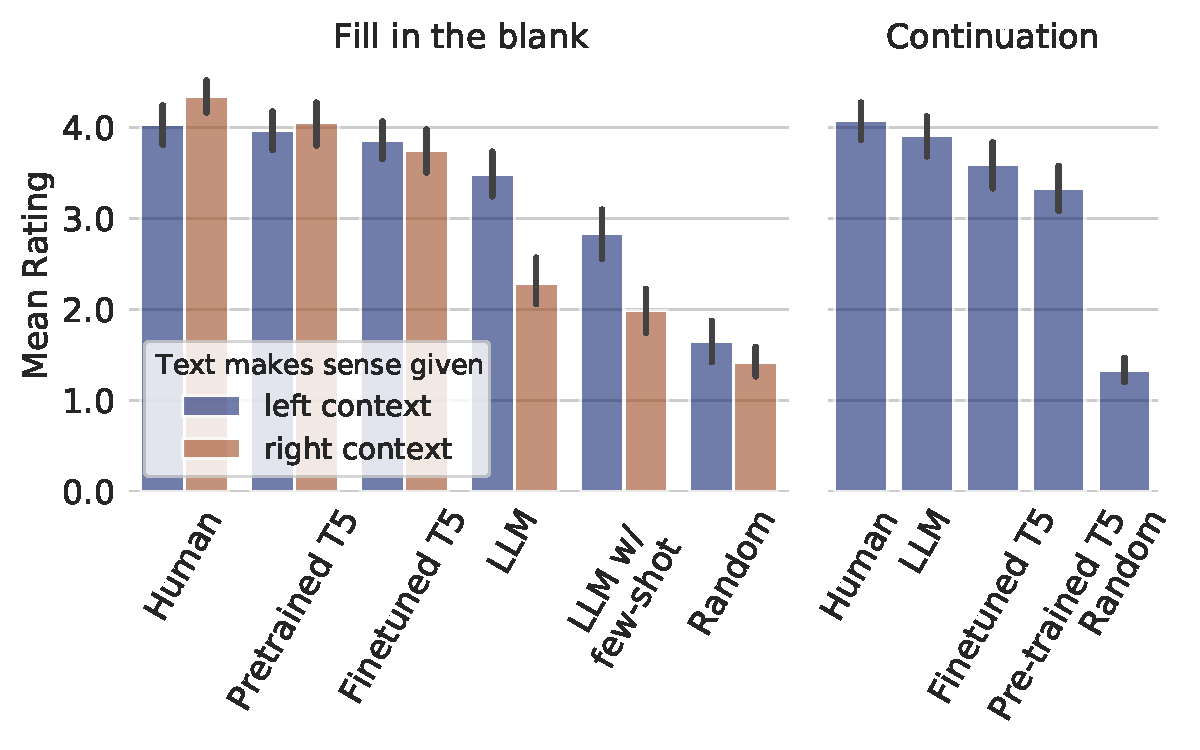
\includegraphics[width=0.49\textwidth, trim={0 0.55cm 0 0}, clip]{figures/human_eval}
    \vspace{-1.75em}
    \caption{Human ratings of \FitB{} generations (left) and continuation generations (right). Error bars are 95\% confidence intervals.}
    \label{fig:human_eval_results}
\end{figure}

\begin{table}[t]
\centering
\small
    \caption{Accuracy of models finetuned on \FITBFITE{} at correctly using provided length and goal conditioning signals. \label{tab:conditioning_signal}}
    \begin{tabular}{p{7em}|rr}
    % & \multicolumn{2}{c|}{XL} \\
    \toprule
    % & \multicolumn{2}{c|}{Large} \\
    \textbf{Finetuned T5} & Context & Length \\
     \midrule
    \cFITB & 0.860 & 0.877 \\
    \rwpFITB & 0.797 & 0.881 \\
    \midrule
    \cFITE & 0.858 & 0.775 \\
    \rwpFITE & 0.791 & 0.746 \\
    \bottomrule
    \end{tabular}
\end{table}

\subsection{Results}
\subsubsection{Difficulty in Developing a Few-Shot Prompt for the Infilling Task}
Filling in a blank seems like a task that ought to be easy to accomplish with few-shot learning techniques.
Training data for large language models often contains fill-in-the-blank style examples, as school lessons with cloze-style questions are relatively common on the internet.
Furthermore, infilling ought to be an easier task tha continuation since there is more information available for the model to base its prediction on.
However, after conducting a large-scale study of many possible few-shot prompts, we found that this technique fell short for the fill-in-the-blank task.


Choosing appropriate examples for a few-shot prompt is very challenging because task performance is often sensitive to minor changes in prompt design \citep{zhao2021calibrate}.
We experimented with prompts randomly selected from the C4, Reddit Writing Prompts, and ROC Stories training sets, as well as prompts consisting of examples we hand-wrote with the goal of story-writing in mind.
For each prompt source, we randomly generated five possible prompts, each with three examples, using the method descrribed in Section \ref{section:few_shot_prompt_selection}.
To simplify the task, we conditioned on desired length but did not include goal conditioning.

An example prompt is shown in Figure \ref{fig:few_shot_prompt}.
When choosing random few-shot prompts from the dataset train sets, in order to keep the few-shot prompt text within the 512-token context length limit of model we used for inference, we only considered examples that contained 100 or fewer tokens, so that the max length of the few-shot prompt was no more than 300 tokens.
This left 212 tokens for the text of the actual example we were interested in performing the \FitB{} task on.
For each evaluation set, examples with inputs longer than 212 tokens were excluded from analysis.
For our hand-written prompt, we wrote the 7 examples shown in Table \ref{tab:custom_examples}.
We generated 5 possible prompts by randomly subsampling 3 examples out of these 7.

\definecolor{lg}{rgb}{0.6,0.6,0.6}

\begin{table}
    \centering
    \small
    \begin{tabular}{|p{0.5\linewidth}|p{0.3\linewidth}|}
         \midrule
         \textbf{Context} & \textbf{Target} \\
         \midrule
An elderly man was sitting alone on a dark path. The man looked down at his feet, and realized \_\_\_\_ . It was a plain pine box and looked as if it had been there for a long time. The man was afraid to look inside the box. & he was holding a bright red box made of pine \\
\arrayrulecolor{lg} \midrule \arrayrulecolor{black}
The mantle was cluttered with objects: \_\_\_\_ and more than one vase of dried flowers. The bejeweled lamp was at the very back, nearly invisible. & picture frames showing grandchildren and long-ago weddings, knickknacks collected from all over the world, \\
\arrayrulecolor{lg} \midrule \arrayrulecolor{black}
"We have to leave now!" Sarah shouted. \_\_\_\_ The only way out was up. We climbed flight after flight. The sound of the monsters banging on the door below became more distant but no less threatening. & "The zombies are going to break through any moment, and then we'll all be goners." \\
\arrayrulecolor{lg} \midrule \arrayrulecolor{black}
The sun was shining, and little gusts of wind brought through the window \_\_\_\_ shocking contrast from the stale city smells she had grown used to. & the faint scents of honeysuckle and freshly turned soil. It was a \\
\arrayrulecolor{lg} \midrule \arrayrulecolor{black}
I was minding my business at the park, when I was approached by a little girl who was crying because she had lost \_\_\_\_ so of course I helped search. & her cat, which she had just received for her birthday. She did not want her parents to know she'd already lost him. I'm a good person \\
\arrayrulecolor{lg} \midrule \arrayrulecolor{black}
It was a cold night, and a storm was raging out at sea. A lightning bolt lit up the sky, briefly illuminating the lighthouse \_\_\_\_ plummeted but just before reaching the churning water, he disappeared in a poof of purple flame! & and the young man peering hesitantly over the sheer cliff. Before the next peal of thunder he jumped. At first he  \\
\arrayrulecolor{lg} \midrule \arrayrulecolor{black}
The magician pulled out of his pocket \_\_\_\_ and then a second one and a third. He didn't stop until soon the ground was covered with them. & a scarlet handkerchief  \\
         \midrule
    \end{tabular}
    \caption{Hand-written fill-in-the-blank examples used for ``custom'' prompt during few-shot learning.}
    \label{tab:custom_examples}
\end{table}



\begin{figure}
    \centering
    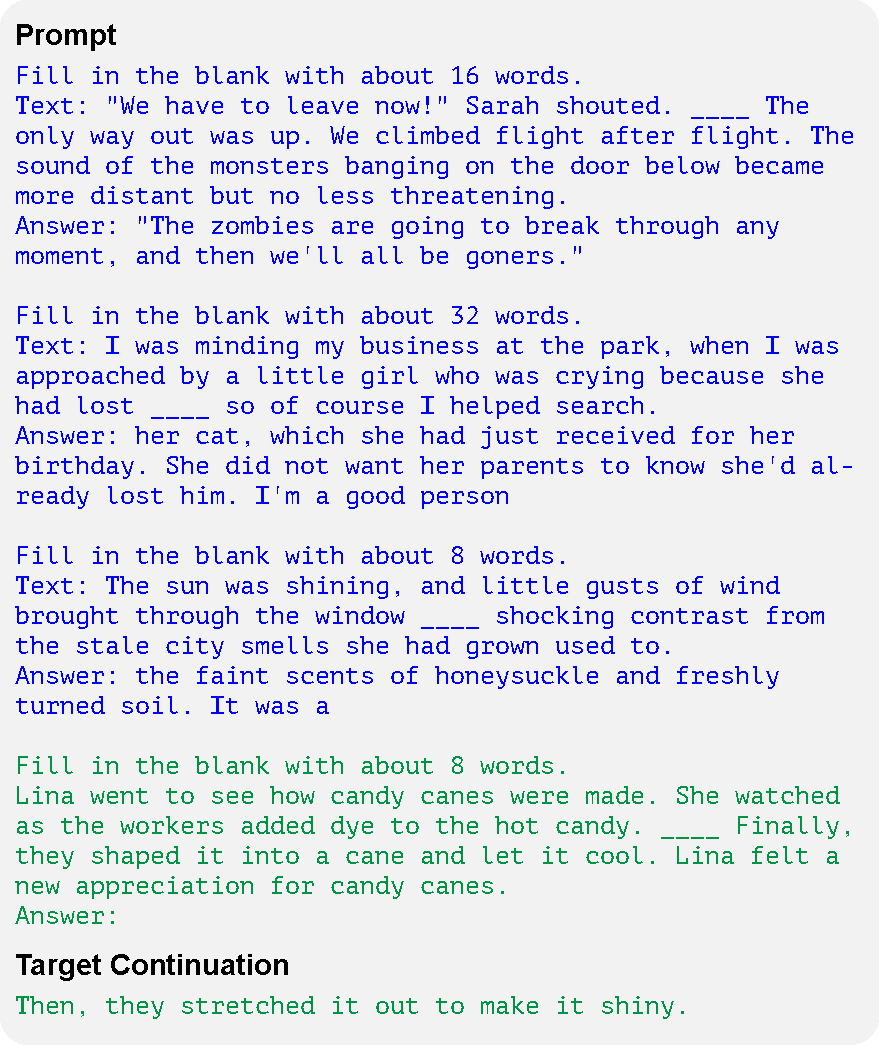
\includegraphics[width=0.48\textwidth]{figures/fsprompt}
    \caption{In blue, one of the few-shot prompts that was derived from handwritten examples, and in green, the target example we would like to perform infilling on.}
    \label{fig:few_shot_prompt}
\end{figure}

Table \ref{tab:generative_ppl_results_full} shows the perplexity of the generations from each few-shot prompt.
We note that even leaving room for 212 tokens worth of context text, some evaluation examples did not fit in the prompt length, and these examples were skipped when doing this analysis.
Figure \ref{fig:skipped_fs_examples} shows a histogram of the fraction of validation set examples that remained for each few-shot prompt after the too-long examples were filtered out.
Based on these results, we chose to include in human evaluation the best few-shot prompt from from \rocFITB and the best few-shot prompt from \cFITB.
Figure \ref{fig:human_eval_results} in the main paper shows the result from the \cFITB few-shot prompt, whose outputs were rated slightly higher by human annotators.

Unfortunately, it is computationally impossible to conduct an exhaustive search of all possible example choices and prompt formats. 
While none of the prompts we tried led to strong performance at the fill-in-the-blank task, we cannot rule out the possibility there might exist a prompt we did not test for which this performance might have been significantly better.
For example, we did not conduct formal experiments to systematically vary the prompt wording/formatting shown in Figure \ref{fig:few_shot_prompt}.
We can conclude that the process of finding an ideal prompt requires time-consuming trial-and-error and is quite difficult!

\begin{figure}
    \centering
    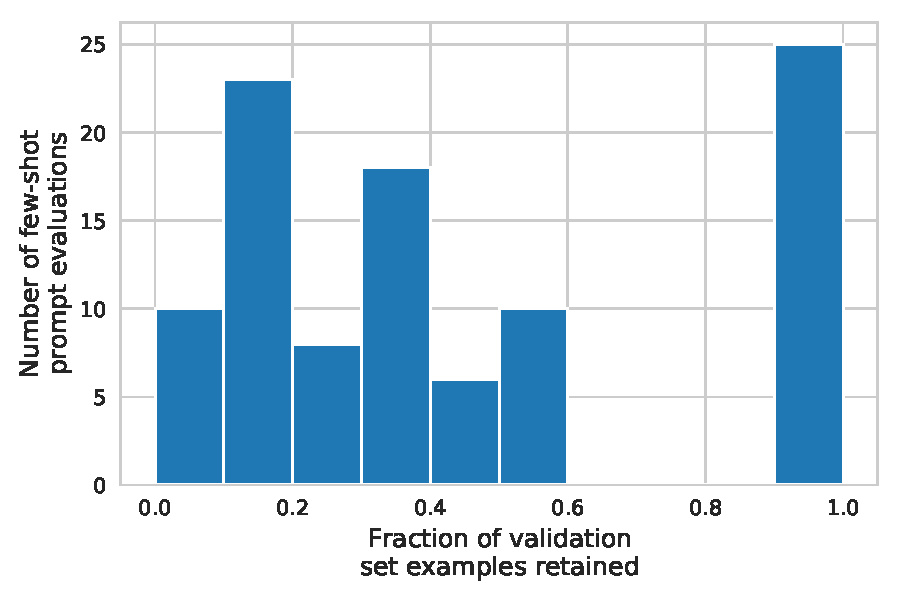
\includegraphics[width=0.49\textwidth]{figures/fs_eval_sets_sizes}
    \caption{For many of the (validation set, few-shot prompt) combinations, not all validation set examples fit into the maximum sequence length for the \LLM.
    The x-axis on this figure is the fraction of validation set examples which were retained after too-long examples were filtered out.
    The y-axis is the count of (validation set, few-shot prompt) pairs.}
    \label{fig:skipped_fs_examples}
\end{figure}

\begin{table}[htbp]
\caption{Perplexity of evaluation sets when the blank has been filled in using \LLM{} with few-shot prompting (top) and  our best fine-tuned T5 model ((bottom).
% Perplexities are averaged over 5 prompts, and
Among the few-shot results, the best method for each dataset is bolded, as well as methods within one standard error.
}
\label{tab:generative_ppl_results_full}
  \centering
  \small
    \begin{tabular}{l|rrrr}
    \toprule
    %  & \cFITB & \rocFITB & \rwpFITB & \rwpFITB-Sent \\
    & \textsc{C4Fill} & \textsc{RocFill} & \textsc{RwpFill} & \textsc{RwpFill} \\
    \textbf{Few-shot source:} & \textsc{Blank} & \textsc{Middle} & \textsc{Blank} & \textsc{Blank}-Sent \\
    \cline{2-5}
    % \midrule
    % \textbf{\cFITB} & 15.67 & \textcolor[rgb]{ 1,  0,  0}{19.72} & \textbf{19.65} & \textbf{16.82} \\
    {\cFITB} & 15.67 & 19.72 & \textbf{19.65} & \textbf{16.82} \\
    {\rocFITB} & \textbf{14.14} & 19.61 & \textbf{19.48} & \textbf{16.36} \\
    {\rwpFITB} & 24.39 & 20.29 & 32.33 & 28.13 \\
    {\rwpFITB-Sent} & 18.91 & \textbf{18.21} & 24.44 & 19.87 \\
    {\textsc{FS Custom}} & 17.98 & 19.80 & 21.72 & 18.38 \\
    \midrule
    {Finetuned T5 XL} & 9.99 & 19.00 & 13.64 & 10.03 \\
    Finetuned T5 Large & 10.33 & 20.47 & 14.08 & 10.37 \\
    % \textbf{\FITB{}  Large} & 10.34 & 20.61 & 14.08 & 10.35 \\
    \bottomrule
    \end{tabular}%
\end{table}

\subsubsection{Automatic Evaluation}
We measure the fluency of proposed generations by evaluating the perplexity of each dataset's examples when the predicted text is placed in the blank \citep{donahue2020enabling}.
We use the \LLM{} to measure perplexity\footnote{Note, since this is the same model being used for generation for our continuation baseline, this metric may be biased.}.
The results are shown in Table \ref{tab:generative_ppl_results}.
We see that the \LLM{} struggles to generate fluent infills, even when used in a few-shot setting.
The only exception to this is ROC Stories, a dataset with fairly simplistic, predictable language.
Finetuning T5 does not result in significantly improved fluency over the pre-trained model except on ROC Stories. 
Lastly, for ROC Stories, we compare against \citet{donahue2020enabling}'s finetuned GPT-2 small, which yielded less fluent predictions.
Table \ref{tab:generative_ppl_continuation_results} shows a similar analysis on our continuation-style datasets. Both T5-based models achieve roughly the same fluency. 

\subsubsection{Human Evaluation}
Human evaluation was conducted on 70 examples, 35 from \rwpFITB{} and 35 from \rwpFITE, with examples about evenly distributed across length buckets.
For \rwpFITB{} evaluation tasks, the rater was presented an input context and several possible sequences that could go in the blank. 
They were asked to rate each sequence first, on how well it fit the text before it, and second, on how well it fit with the text following it, according to a 5-point slider 
For \rwpFITB{}, the task was almost the same, except that the rater was presented only a left context and asked to rate how well it continued the prompt.
A screenshot of the Human Intelligence Task (HIT) used for annotations is shown in Figure \ref{fig:amturk_ui}. Workers were paid originally paid \$1.85 per HIT, but since the average HIT duration ended up being 15 minutes, we awarded each rater a bonus to raise their pay to an average of \$10 per hour.
Each example was shown to three raters, and annotations were rejected if the rater gave a lower overall score to the random output than to the ground-truth one.
A total of 3 annotations were rejected.
Overall, the Fleiss' kappa agreement of pairs of annotators giving the same numerical score to the same question was 0.26.

\begin{figure}[ht]
    \centering
    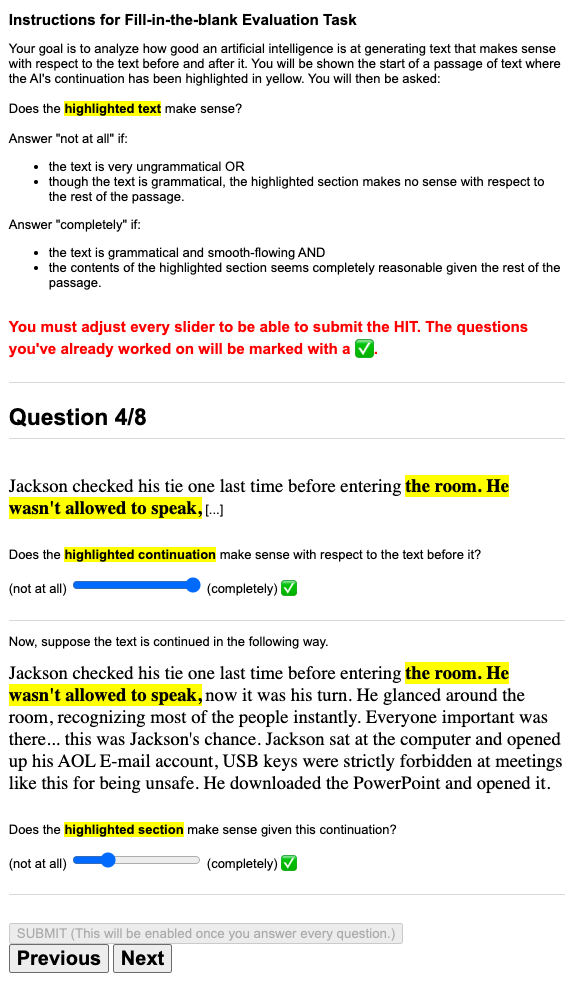
\includegraphics[width=0.49\textwidth, frame]{figures/amt_screenshot.png}
    \caption{A screenshot of the question structure for human evaluation.}
    \label{fig:amturk_ui}
\end{figure}

Figure \ref{fig:human_eval_results} shows the results.
On the \FitB{} task, the pre-trained and finetuned T5 models were indistinguishable in terms of quality.
The \LLM{} that formed continuations prompted with only the left context did somewhat better than the few-shot \LLM{}, indicating that few-shot learning is not yet a feasible alternative to finetuning.
On the continuation task, the \LLM{} has the highest rating, which is unsurprising since it is a much larger model than T5.
However, the finetuned T5 is rated almost as highly.
Overall, these results suggest that T5, unlike the \LLM{}, can be used effectively for continuation as well as \FitB.
Furthermore, if one doesn't care about controllability, T5 can be used effectively for both tasks without any finetuning.

\subsubsection{Benefits of Controllability}
% The biggest problem with using pre-trained T5 is the lack of controllability.
There are good reasons to care about controllability.
For example, length conditioning is extremely important for \FitB models, since it is not possible to control the generation length by simply sampling more or fewer tokens.
Pre-trained T5 tends to produce infill proposals which are shorter than the groundtruth (Figure A\ref{fig:t5_lengths}), and there is no way to ask the model to produce longer generations.
In contrast, finetuned T5 was able to produce generations in the target length bucket over 74\% of the time (Table \ref{tab:conditioning_signal}).
% ldugan: This is really interesting, I wonder how many of the prompts were within one bucket of the desired length? I think that number might be a bit more telling
Goal conditioning, while not strictly necessary for either either task, has been shown to be useful for generative commonsense reasoning \citep{lin2020commongen} and may empower users in downstream applications such as AI-assisted creative writing \citep{roemmele2021inspiration}. 
Finetuned T5 is able to use all of the specified goal words over 79\% of the time.


\begin{figure}
    \centering
    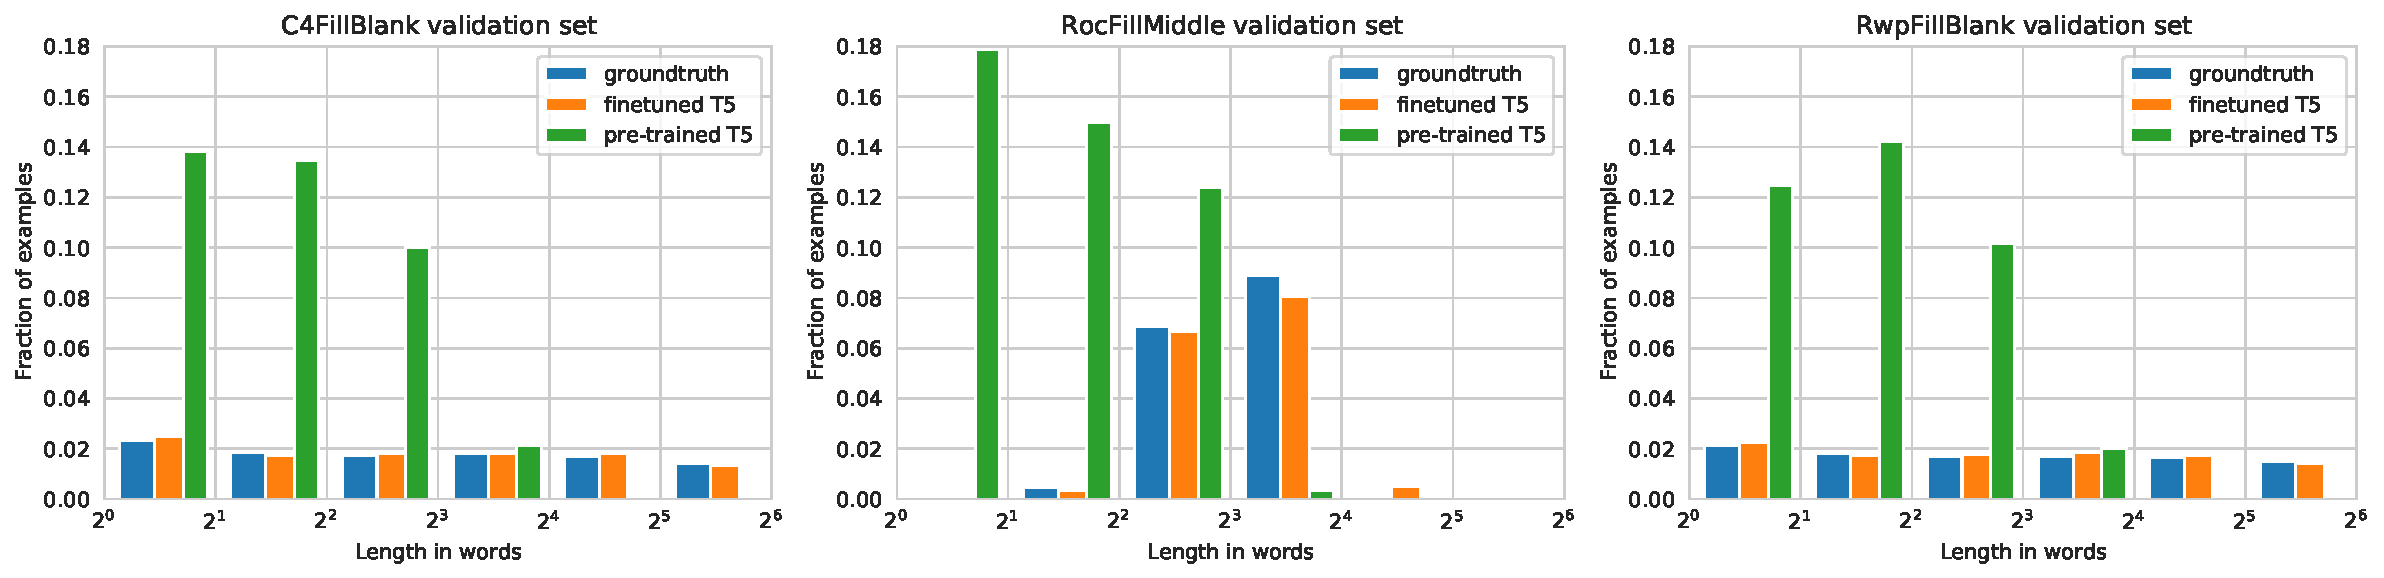
\includegraphics[width=0.8\textwidth]{figures/t5_lengths}
    \caption{For each of the \FitB{} validation sets, a histogram of the distribution of sequence lengths (measured in words) of the {groundtruth} blanked out text and the proposed infills from T5 {after} and {before} finetuning). We see that pre-trained T5 tends to produce text that is shorter than the groundtruth.}
    \label{fig:t5_lengths}
\end{figure}

\subsubsection{Domain Transfer}
Prior work on \FitB{} tends to only evaluate models trained on data from the same domain as the validation set.
Our results show that despite training exclusively on C4, T5 models have strong transferability to more targeted domains such as Reddit Writing Prompts.
This sort of transferability is extremely important for achieving the goal of having single models which can handle many tasks and domains.

\subsection{Conclusion}
In this work, we make the case for starting with a model capable of filling in the blank when attempting to build a system that can perform both \FitB{} and continuation.
As LMs become bigger, it will be unsustainable to have separately trained models per task.
Multi-task, domain-transferable models with like the ones we propose require less total training and are more efficient to store and use at inference time.
While pre-trained T5 by itself is capable of both infilling and continuation, additional conditioning signals such as desired length and goal text can be successfully incorporated into fine-tuning in order to support an even greater diversity of model interactions.
Finally, we present a negative result that while few-shot learning is a promising method for
building multi-task support without any finetuning, it is challenging to make work for the \FitB{} task. 

% Takeaway 1: Fill-in-the-blank models can effectively do both fill-in-the-blank and continuation.
% Takeaway 2: Few-shot learning is not effective for the fill-in-the-blank task.
% Takeaway 3: Fine-tuning explicitly for fill-in-the-blank is only necessary if you want extra controllability.

% Point out any strong assumptions and how robust your results are to violations of these assumptions (e.g., independence assumptions, noiseless settings, model well-specification, asymptotic approximations only held locally). Reflect on how these assumptions might be violated in practice and what the implications would be.
% Reflect on the scope of your claims, e.g., if you only tested your approach on a few datasets, languages, or did a few runs. In general, empirical results often depend on implicit assumptions, which should be articulated. Reflect on the factors that influence the performance of your approach. For example, a speech-to-text system might not be able to be reliably used to provide closed captions for online lectures because it fails to handle technical jargon.
% If you analyze model biases: which definition of bias are you using? Did you state the motivation and definition explicitly? See the discussion in Blodgett et al. (2020).
% We understand that authors might fear that complete honesty about limitations might be used by reviewers as grounds for rejection. It is worth keeping in mind that a worse outcome might be if reviewers discover limitations that aren’t acknowledged in the paper. In general, we advise authors to use their best judgement and recognize that individual actions in favor of transparency play an important role in developing norms that preserve the integrity of the community. Reviewers will be specifically instructed to not penalize honesty concerning limitations.
% A2. Did you discuss any potential risks of your work?

% Examples of risks include potential malicious or unintended harmful effects and uses (e.g., disinformation, generating fake profiles, surveillance), environmental impact (e.g., training huge models), fairness considerations (e.g., deployment of technologies that could further disadvantage or exclude historically disadvantaged groups), privacy considerations (e.g., a paper on model/data stealing), and security considerations (e.g., adversarial attacks). See discussion in Leins et. al. (2020) as examples.
% Does the research contribute to overgeneralization, bias confirmation, under or overexposure of specific languages, topics, or applications at the expense of others? See Hovy and Spruit (2016) for examples.
% We expect many papers to be foundational research and not tied to particular applications, let alone deployments. However, we encourage authors to discuss potential risks if they see a path to any positive or negative applications. For example, the authors can emphasize how their systems are intended to be used, how they can safeguard their systems against misuse, or propose future research directions.
% Consider different stakeholders that could be impacted by your work. Is it possible that research benefits some stakeholders while harming others? Does it pay special attention to vulnerable or marginalized communities? Does the research lead to exclusion of certain groups? See Dev et. al (2021) for examples.
% Consider dual use, i.e, possible benefits or harms that could arise when the technology is being used as intended and functioning correctly, benefits or harms that could arise when the technology is being used as intended but gives incorrect results, and benefits or harms following from (intentional or unintentional) misuse of the technology.
% Consider citing previous work on relevant mitigation strategies for the potential risks of the work (e.g., gated release of models, providing defenses in addition to attacks, mechanisms for monitoring misuse, mechanisms to monitor how a system learns from feedback over time, improving the efficiency and accessibility of NLP).

\subsection{Summary of Contributions}
The work described in this section was published in the 2022 Proceedings of the North American Association of Computational Linguistics \TODO{citation}.
The work was performed with my collaborators Daphne Ippolito, Liam Dugan, Emily Reif, Ann Yuan, Andy Coenen, and Chris Callison-Burch.
I led this project, designed and ran all experiments, and performed most of the analysis.

\section{Supporting Arbitrary Style Transfer}
\label{section:style_transfer}

Text style transfer is the task of rewriting text to incorporate additional or alternative stylistic elements while preserving the overall semantics and structure.
% Although style transfer has garnered increased interest due to the success of deep learning, these approaches usually require a substantial amount of labeled training examples, either as parallel text data \citep{zhu-etal-2010-monolingual,rao-tetreault-2018-dear} or non-parallel text data of a single style. \citep{li-etal-2018-delete,jin-etal-2019-imat, liu2020revision,style-transfer-as-paraphrase-2020}. 
Early approaches to style transfer required \textit{parallel} text data \citep{zhu-etal-2010-monolingual,rao-tetreault-2018-dear}, where every input in the source style has a corresponding output in the target style.
Because the availability of such data is limited, however, there has been a shift toward approaches which instead rely on \textit{non-parallel} monostyle data \cite{li-etal-2018-delete,jin-etal-2019-imat, liu2020revision,style-transfer-as-paraphrase-2020}.
% % (no mapping between source and target style sentences)
Most recently, \textit{label-free} methods have taken advantage of the natural manifold of language to train style transfer models that require only a few exemplars in the target style for inference \citep{DBLP:journals/corr/abs-1905-11975, DBLP:journals/corr/abs-2010-03802}.
This is true even for approaches which claim to be label-free \citep{DBLP:journals/corr/abs-1905-11975,DBLP:journals/corr/abs-2010-03802}.
Hence, there is a clear need for new methods that both reduce the training data requirements and expand the scope of styles supported \citep{DBLP:journals/corr/abs-2011-00416,DBLP:journals/corr/abs-2010-12742}.

\begin{figure}[t]
     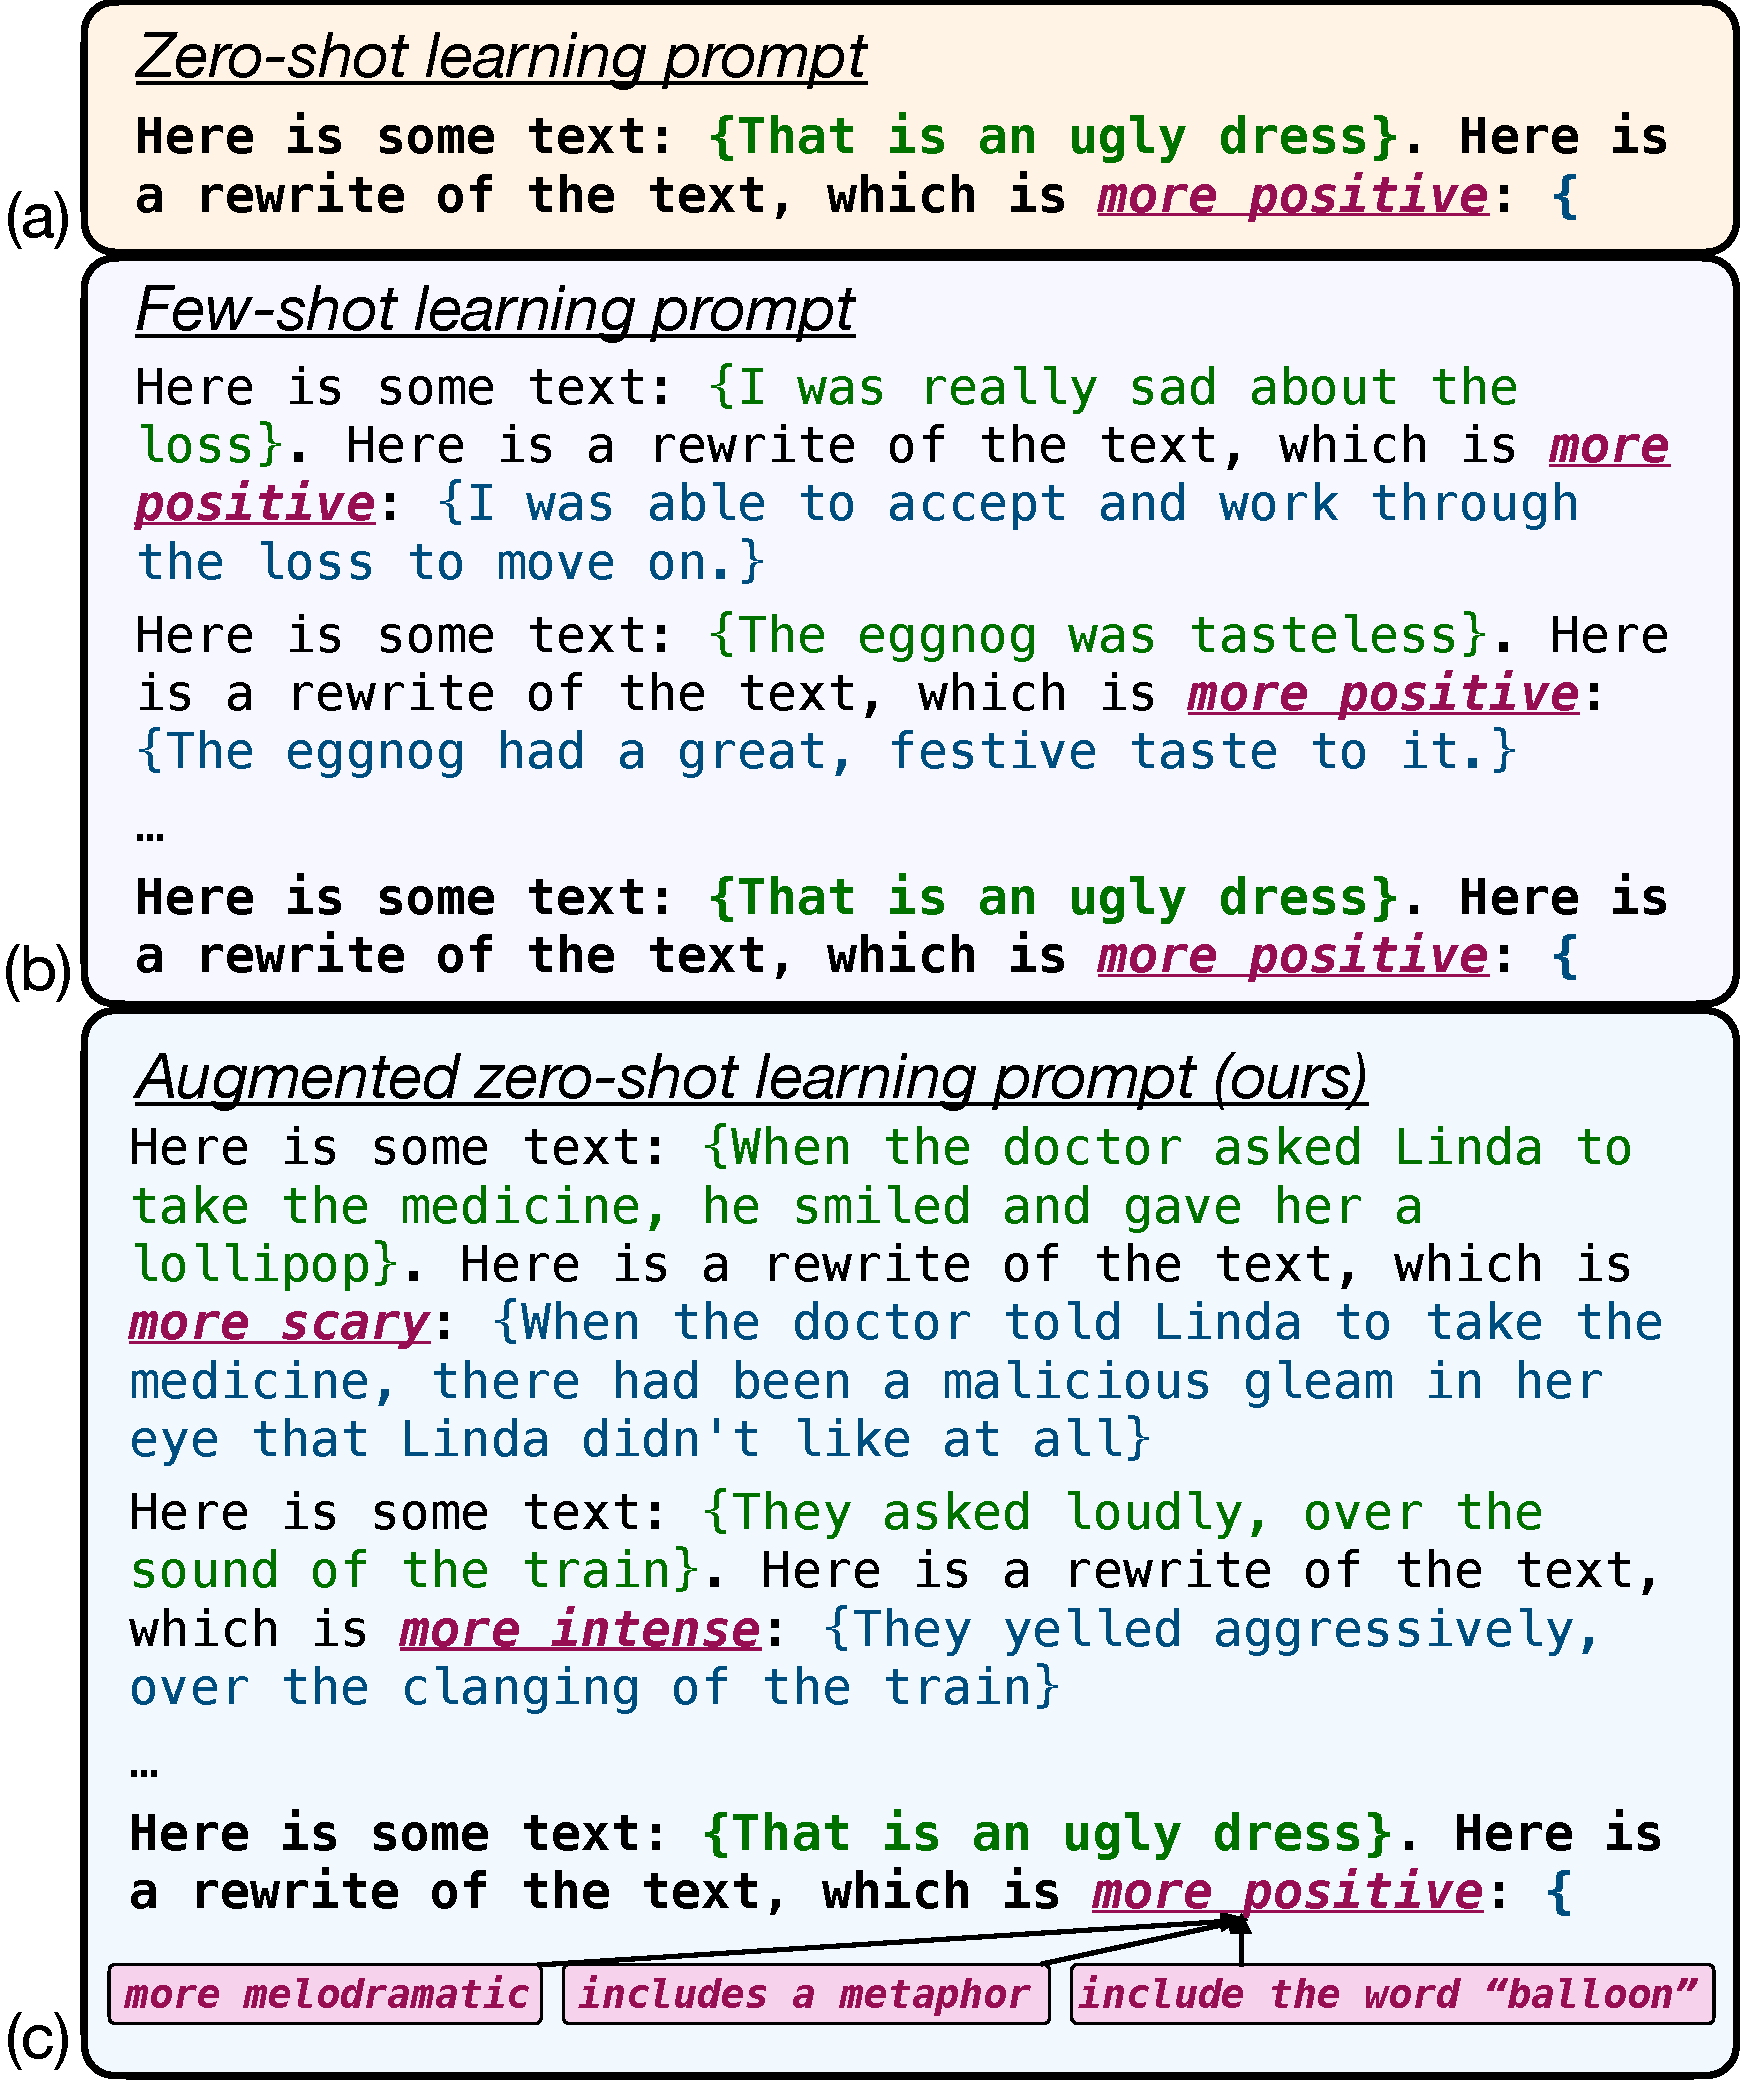
\includegraphics[width=0.99\linewidth]{figures/style-transfer-prompt.pdf}
     \vspace{-1.5mm}
  \caption{Zero-shot, few-shot, and augmented zero-shot prompts for style transfer. The boldface text is the zero-shot prompt, and the plain text is the additional priming sequence. The full prompts used in this paper are shown in Table \ref{tab:fullprompt}. We encourage readers to examine the outputs of our model at \url{https://bit.ly/3fLDuci}.}
  \label{prompts}
\vspace{-3.5mm}
\end{figure}


In this section, we present \textit{augmented zero-shot learning}, a prompting method that allows large language models to perform text style transfer to arbitrary styles, without any exemplars in the target style.
Our method builds on prior work showing that sufficiently large LMs such as GPT-3 can perform various tasks ranging from classification to translation, simply by choosing a clever prompt to prepend to the input text for which the model is asked to continue \citep{DBLP:journals/corr/abs-2005-14165,branwen2020gpt}. 
Although large LMs are trained only for continuation, recent work has shown that they can perform a variety of NLP tasks by expressing the task as a prompt that encourages the model to output the desired answer as the continuation \citep{liu2021pre,puri2019zero,weller-etal-2020-learning,DBLP:journals/corr/abs-2005-14165,schick-schutze-2021-just}. 
The simplest approach, \textbf{zero-shot prompting}, directly uses natural language to ask the large LM to perform a task, as shown in Figure \ref{prompts}a. Zero-shot learning, however, can be prone to failure modes such as not returning well-formatted or logical outputs (see $\S$\ref{section:limitations}).
 However, zero-shot prompts are prone to failure modes such as not returning a well formatted or logical answer.
This problem can often be overcome by prepending exemplars to the prompt that demonstrate what successful completions may look like.
This approach, called \textbf{few-shot prompting}, has been shown to achieve higher performance, but requires exemplars for the exact task that we want the model to perform (Figure \ref{prompts}b).

To remove the need for these labeled exemplars for each style transfer task, we propose \textit{augmented zero-shot learning}, a method for performing multi-task style transfer using a single set of exemplars.
Instead of prompting the model with exemplars specific to the exact style transfer task we wish to perform, we prompt the model with examples of a variety of sentence rewriting operations, as shown in Figure \ref{prompts}c. 
This intuition is inspired by \citet{reynolds2021prompt}'s observation that successful prompts constrain the behavior of the large LM away from failure modes---in our case, we aim to preserve the flexibility of a zero shot prompt while encouraging the model to produce outputs of a specific template.
We keep the the format of the exemplars constant and insert the desired sentence transformation into the same format.
In this way, the augmented zero-shot formulation supports arbitrary sentence rewriting tasks without the need to write any task-specific exemplars.
Thus, it works for a wide range of styles, including modifying the text to be ``\textit{more melodramatic,}'' ``\textit{insert a metaphor,}'' or ``\textit{include the word balloon.}''

Augmented zero-shot learning is simple and facilitates the application of style transfer to a wider range of styles than existing work.
We also foresee that our strategy of prompting an LLM with non-task specific examples will prove useful for other tasks besides style transfer.

\subsection{Experimental Setup}

\begin{table}[]
    \caption{Example style transfer outputs from augmented zero-shot learning for non-standard styles. }  %See all our outputs at \url{https://bit.ly/3fLDuci}
  \label{tab:style-transfer-examples}%
\setlength{\tabcolsep}{3.3pt}
  \small
    \label{fig:visualizer_results}
    \begin{tabular}{p{0.25\linewidth}>{\scriptsize}p{0.7\linewidth}}
    \toprule
    Original & \texttt{There, in the middle of the street, stood an old man in a weatherbeaten brown coat.} \\
    \hline
    More\newline descriptive &
    \texttt{The man's brown trenchcoat was coated with snow, and as he leaned against the telephone booth, he cast a long shadow across the road in the late afternoon sun.}\\
    \hline
    Include a\newline metaphor &
    \texttt{There, in the middle of the street, stood an old man whose face resembled the weatherworn bark of a gnarled tree.}\\
    \hline
    Include the \newline word ``\textit{park}'' & \texttt{There, in the middle of Central Park, stood an old man in a weatherbeaten brown coat.} \\
    \hline
    Include the \newline word ``\textit{balloon}'' & \texttt{There, in the middle of the street, stood an old man with several colourful balloons tied to the straps of his coat.} \\
    \hline
    More comic & \texttt{There, in the middle of the street, stood an old man in a raggedy brown coat that was much too big for him.} \\
    \hline
    More melodramatic & \texttt{There, in the middle of the road, stood a grizzled old man, the light of life faded from his sunken eyes.}\\
    \bottomrule
    \end{tabular}%
    \vspace{-1mm}
\end{table}%






% \begin{table*}[tbp]
%   \small
%     \label{fig:visualizer_results}
%     \begin{tabular}{p{0.12\linewidth}>{\tiny}p{0.4\linewidth}>{\tiny}p{0.4\linewidth}}
%     \toprule
%     Original & \texttt{There, in the middle of the street, stood an old man in a weatherbeaten brown coat.} & \texttt{There was a large metal desk pressed against a wall.} \\
%     \hline
%     More\newline descriptive &
%     \texttt{The man's brown trenchcoat was coated with snow, and as he leaned against the telephone booth, he cast a long shadow across the road in the late afternoon sun.} &
%     \texttt{The large metal desk was bolted into the floor behind reinforced steel and a thick layer of concrete, with a small blinking red light that was the only thing not covered in dust.} \\
%     \hline
%     Include a\newline metaphor &
%     \texttt{There, in the middle of the street, stood an old man whose face resembled the weatherworn bark of a gnarled tree.}&
%     \texttt{The desk was like a gray fortress.} \\
%     \hline
%     Include the \newline word ``park'' & \texttt{There, in the middle of Central Park, stood an old man in a weatherbeaten brown coat.} & \texttt{There was a large green metal desk at the entrance of the park.} \\
%     \hline
%     Include the \newline word ``balloon'' & \texttt{There, in the middle of the street, stood an old man with several colourful balloons tied to the straps of his coat.} &
%     \texttt{There was a large metal desk pressed against a wall. On it was a cluster of large, red balloons.} \\
%     \hline
%     More comic & \texttt{There, in the middle of the street, stood an old man in a raggedy brown coat that was much too big for him.} &
%     \texttt{There was a round little table with a little lamp on it pressed against a wall that was decorated with a bunch of little knick-knacks for decoration.} \\
%     \hline
%     More melodramatic & \texttt{There, in the middle of the road, stood a grizzled old man, the light of life faded from his sunken eyes.} &
%     \texttt{There was a resounding, metalic CLANG echoing through the hallway. It made me jump. When I looked, I saw a large desk that was placed on the floor, pressed up against one of the walls.} \\
%     \bottomrule
%     \end{tabular}%
%     \caption{Two examples of style transfer with augmented zero shot learning to several different different styles. See all our outputs, including baselines and prior methods at \url{https://bit.ly/3fLDuci} \TODO{finalize ui}} 
%   \label{tab:style-transfer-examples}%
% \end{table*}%

\subsubsection{Style Transfer Tasks}
% \label{section:tasks}
% We evaluate augmented zero-shot prompting on a number of text style transfer tasks.
We consider six style transfer tasks that we deem non-standard, listed in Table \ref{tab:style-transfer-examples}.
These styles were chosen to be representative of most frequent style adjustments made by users of an AI-assisted text editor that employs our method (discussed further in $\S$\ref{subsec:potential}). 
As source sentences, we use 50 sentences randomly drawn from the Reddit Writing Prompts validation set \citep{fan2018hierarchical}, excluding those that already clearly exhibited one of the styles or were ungrammatical/incoherent.
We use human evaluation for these styles, since not all styles have readily available classifiers.
% For input sentences, we draw a random set of 50 sentences\footnote{We only evaluate 50 sentences because style transfer for arbitrary styles can only be evaluated manually, and we have many styles and models (totaling 7200 ratings.)} from short stores in the Reddit Writing Prompts validation set \citep{fan2018hierarchical}, excluding sentences that were incoherent or clearly exhibited one of the styles already. 

We also evaluate our method on two standard style transfer tasks: sentiment and formality.
We use the Yelp polarity dataset \citep{zhangCharacterlevelConvolutionalNetworks2015} for sentiment and Grammarly's Yahoo Answers Formality Corpus (GYAFC) dataset for formality \citep{rao-tetreault-2018-dear}.\footnote{Hosted by \citet{DBLP:conf/ijcai/LuoLZYCSS19}.}
These datasets allow us to evaluate performance of augmented zero-shot learning in the context of prior supervised methods which have been used on these tasks.

\subsubsection{Model}
\label{subsection:lambda_description}
Augmented zero-shot learning requires a large language model.
We primarily use LaMDA, a left-to-right decoder-only transformer language model \citep{DBLP:journals/corr/VaswaniSPUJGKP17} with a non-embedding parameter count of 137B \citep{thoppilan2022lamda}. 
The pre-trained LaMDA model, which we refer to as \textit{LLM}, was trained on a corpus comprising 1.95B public web documents, including forum and dialog data and Wikipedia.
The dataset was tokenized into 2.49T BPE tokens with a SentencePiece vocabulary size of 32K \citep{DBLP:journals/corr/abs-1808-06226}.
We also use \textit{LLM-Dialog}, the final LaMDA model which was finetuned on a curated, high-quality subset of data identified to be in a conversational format.
Decoding was done with top-$k$=40.
To show that the success of augmented zero-shot learning is not restricted to these two large LMs, we also perform experiments with GPT-3 (Table \ref{tab:candidate_select}).
For GPT-3, decoding was done with nucleus sampling using $p$=0.6 \citep{holtzman2019curious}.

The full prompts used for \textit{LLM} and GPT-3 are shown in Figure \ref{tab:fullprompt}.
For \textit{LLM-Dialog}, the prompt was instead formulated as a conversation between one agent who is requesting rewrites and another who is performing the rewrites.

% \subsection{Evaluation}
% We evaluate the quality of our style transfers on three main axes.

% \begin{enumerate}[nolistsep]
%     \item \textbf{Transfer strength} is the amount that the output actually matches the desired target style. 
%     \item \textbf{Semantic preservation} is the similarity between the input and output texts: that is, the amount that the output text's underlying meaning and structure matches that of the input. This can be difficult to measure, as the style may change the attributes by definition. For example, if the original text is ``this restaurant is terrible'' and the style is ``have a more positive sentiment'', then the underlying meaning of the sentence will necessarily change.
%     \item \textbf{Fluency} is a measure of whether the text's coherence, i.e., whether it could have been written by a proficient English speaker.
% \end{enumerate}

% We evaluate with human raters to compare our method against baselines and prior methods. Additionally, we use automatic evaluation for the task of sentiment transfer to compare across a larger number of prior approaches and variations of our augmented zero-shot recipe.
% % As \citet{DBLP:journals/corr/abs-2010-12742} discuss, automatic evaluation for style transfer is a difficult problem since the domain is so subjective, and metrics calculated automatically do not always match human baselines.
% % Despite these caveats, automatic evaluation is ubiquitous in prior work.

% The outputs used for human evaluation were generated using augmented zero shot learning on LLM-dialog, with no candidate selection.
% For each input sentence and target style, raters were shown several possible outputs and asked to rate each (\textit{input}, \textit{style}, \textit{output}) tuple along the three axes of transfer strength, semantic preservation, and fluency.
% Each question was assigned to three different raters.
% Screenshots of the rater UI are shown in figure \ref{fig:rater_ui} in the Appendix. 

% For automatic evaluation, we evaluate transfer strength with the built-in sentiment classification model from HuggingFace \citep{wolf-etal-2020-transformers}, semantic preservation measured with BLEU \citep{papineni2002bleu}, and fluency (measured by perplexity with according to GPT-2, 117M) following \citet{DBLP:journals/corr/abs-2011-00416, DBLP:journals/corr/abs-2010-12742}.


\subsection{Results}
\subsubsection{Non-Standard Styles}
For our six non-standard styles, we asked six professional raters to assess  <input sentence, target style, output sentence> tuples. These raters are fluent in English, live in India, and work full time labeling and evaluating data. To decrease inter-rater discrepancy and ensure that our instructions were clear, we had an initial calibration session where they test-rated a small portion of the data (around 10 datapoints which were then omitted from the results) and asked us any clarifying questions. For each style, we compare outputs from our method plus the three baselines for 50 sentences.


Each tuple was scored by three raters (3,600 ratings total) on the following three axes which are standard to textual style transfer \citep{DBLP:journals/corr/abs-1904-02295}: \textbf{(1) transfer strength} (the amount that the output actually matches the target style), \textbf{(2) semantic preservation} (whether the underlying meaning of the output text, aside from style, matches that of the input), and \textbf{(3) fluency} (whether the text is coherent and could have been written by a proficient English speaker). Following \citet{sakaguchi-van-durme-2018-efficient}, transfer strength and semantic preservation were rated on a scale from 1--100. A screenshot of the evaluation UI is shown in Figure \ref{fig:rater_ui}.
We use \textit{dialog-LLM}, and compare it with three other methods: \textbf{(1) zero-shot} (a baseline), \textbf{(2) paraphrase} (our normal augmented zero shot prompt, but with the target style of \textit{``paraphrased''}, as a control) and \textbf{(3) human} (ground-truth transformations written by the authors).

\begin{figure}[!htb]
  \centering
  \fbox{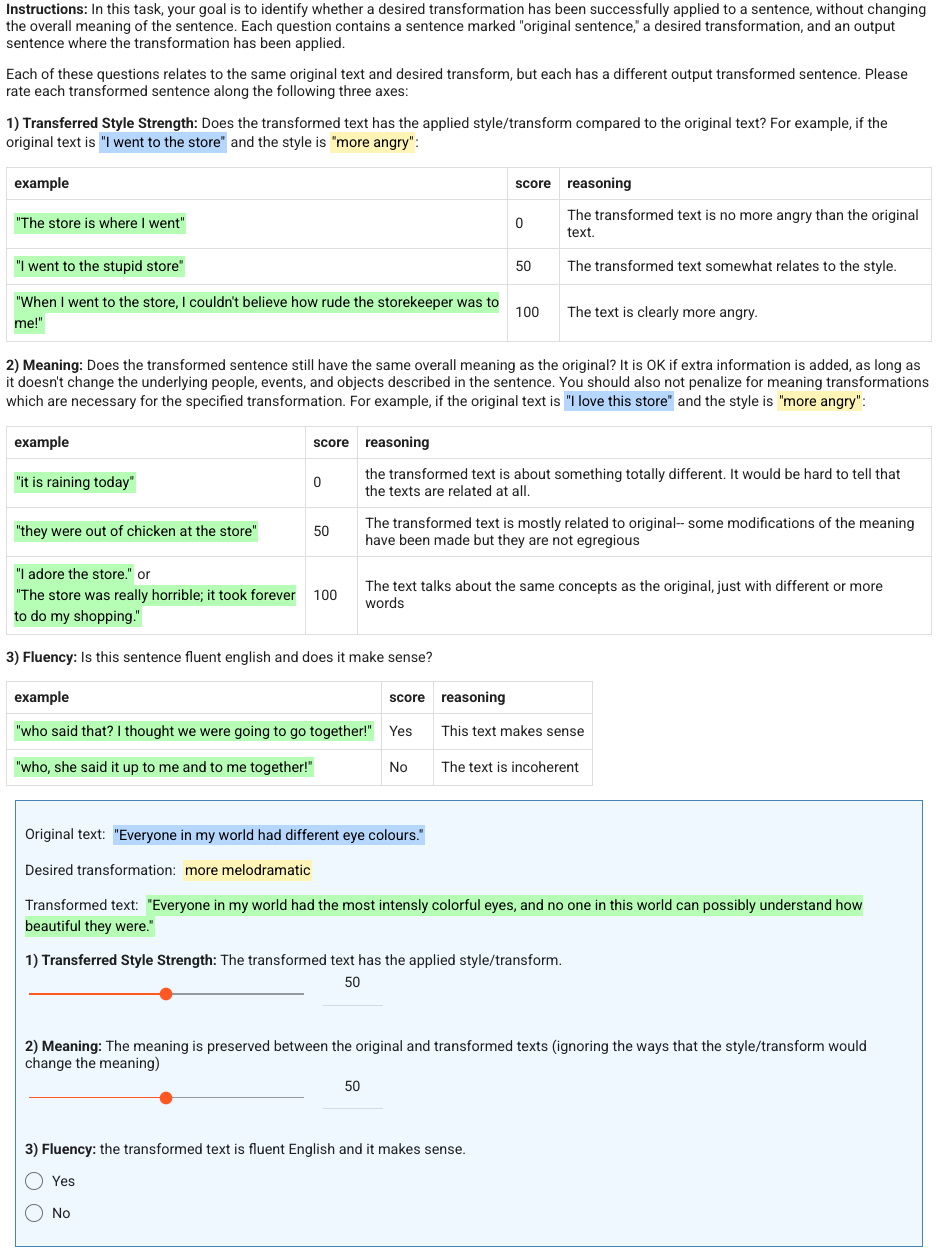
\includegraphics[width=1\linewidth]{figures/rater_ui.png}}
  \caption{The rating UI used for human evaluation. The user may be shown a number of blue squares at once with the same original text and different outputs.}
  \label{fig:rater_ui}
\end{figure} 

Figure \ref{human_eval_other_styles} shows these results. %, and all raw outputs can be found at \url{https://bit.ly/3fLDuci}.
We found that the outputs of our method were rated almost as highly as the human-written ground truth for all three evaluations. The zero-shot baseline performed the worst in all categories: 25.4\% of the time, it did not return a valid response at all (see $\S$\ref{section:limitations}), compared with 0.6\% for augmented zero shot.
The strong performance of the paraphrase baseline at fluency and semantic similarity shows that large LMs are capable of generating high quality text that remains true to the input sentence's meaning.
Overall, the average length of the input sentences was 66 characters, whereas the average length of augmented zero-shot outputs was 107 characters. For context, human paraphrase outputs were 82 characters.
\begin{figure}
    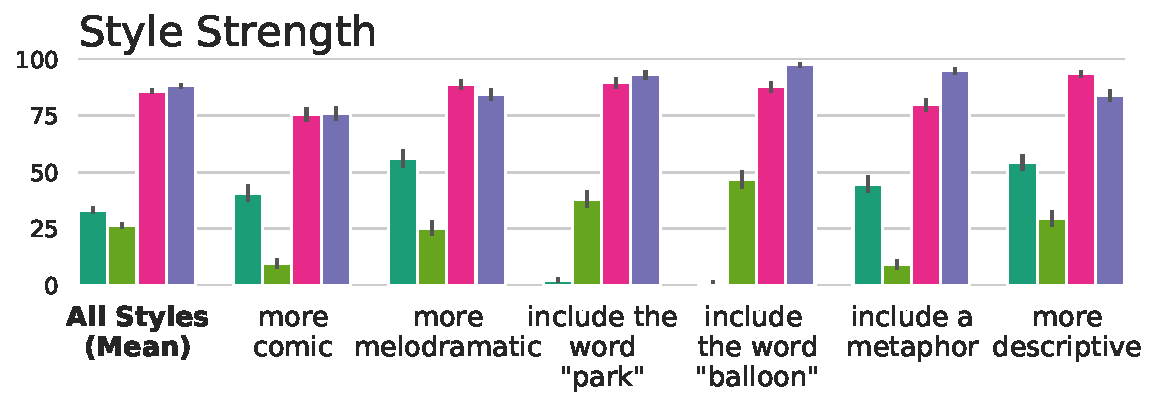
\includegraphics[width=\linewidth]{figures/style_standard_False.pdf}
    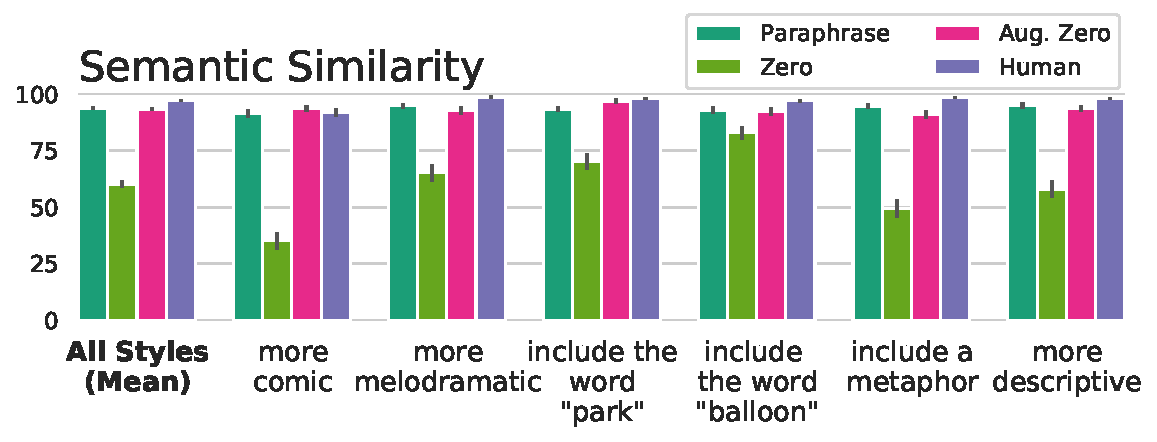
\includegraphics[width=\linewidth]{figures/meaning_standard_False.pdf}
  \vspace{-0.7cm}
  \caption{Human evaluation of style transfer for six atypical styles. Our method is rated comparably to the human-written ground truth. Error bars are mean standard error.}
  \label{human_eval_other_styles}
\end{figure}

For a subset of the tasks, some automatic evaluation was also possible.
We found that the ``\textit{balloon}'' and ``\textit{park}'' transformations successfully inserted the target word 85\% of the time.
% The word ``\textit{park}'' was used in a variety of senses, including``\textit{parking a car}'' and ``\textit{nature park}.'' 
For ``\textit{more descriptive}'' and ``\textit{include a metaphor}'' the transformed text was, as expected, longer than the original (by 252\% and 146\% respectively, compared with 165\% and 146\% for human baselines).

\subsubsection{Standard Styles}
To better contextualize the performance of our method with prior methods, we also generated outputs for two standard style transfer tasks: sentiment and formality. 
Figure \ref{human_eval_standard_style} shows human evaluations (same setup as before) for our outputs as well as the outputs from two popular prior style transfer methods, Unsup MT \citep{prabhumoye-etal-2018-style} and Dual RL \citep{DBLP:conf/ijcai/LuoLZYCSS19}.
The outputs from our method were rated comparably to both human generated responses and the two prior methods, using the same rating setup as the non-standard styles, with six outputs and baselines for four styles across 50 sentences, rated independently by three raters, totalling 3,000 total ratings.

Furthermore, following \citet{li-etal-2018-delete} and \citet{sudhakar-etal-2019-transforming}, we perform automatic evaluation for sentiment style transfer since there are classifiers available for these styles. We note that although automatic evaluations can diverge from human ratings, they can still be a good proxy as we could not perform human evaluation against every prior method due to time and resource constraints.
We automatically evaluate \textbf{(1) transfer strength} using a sentiment classifier from HuggingFace Transformers \citep{wolf-etal-2020-transformers}, \textbf{(2) semantic similarity} to human examples provided by \citet{DBLP:conf/ijcai/LuoLZYCSS19} via BLEU score, and \textbf{(3) fluency} via perplexity, as measured by GPT-2 (117M).

\begin{figure}[t]
    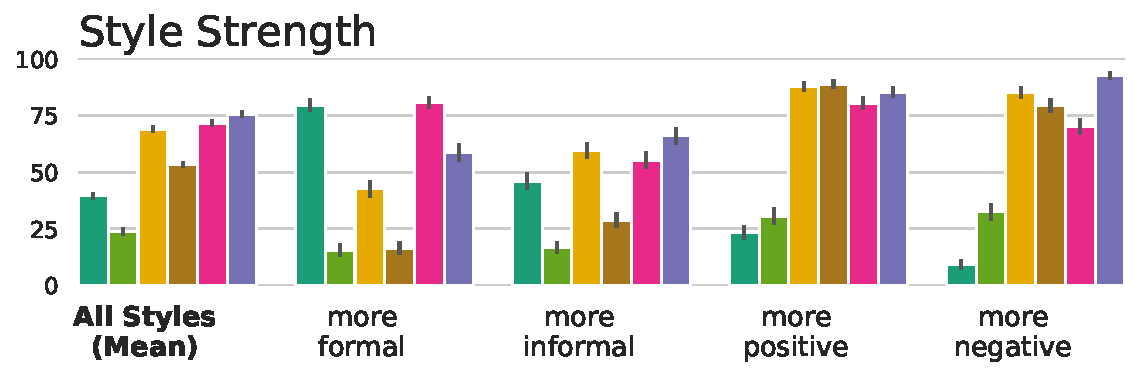
\includegraphics[width=\linewidth]{figures/style_standard_True.pdf}
    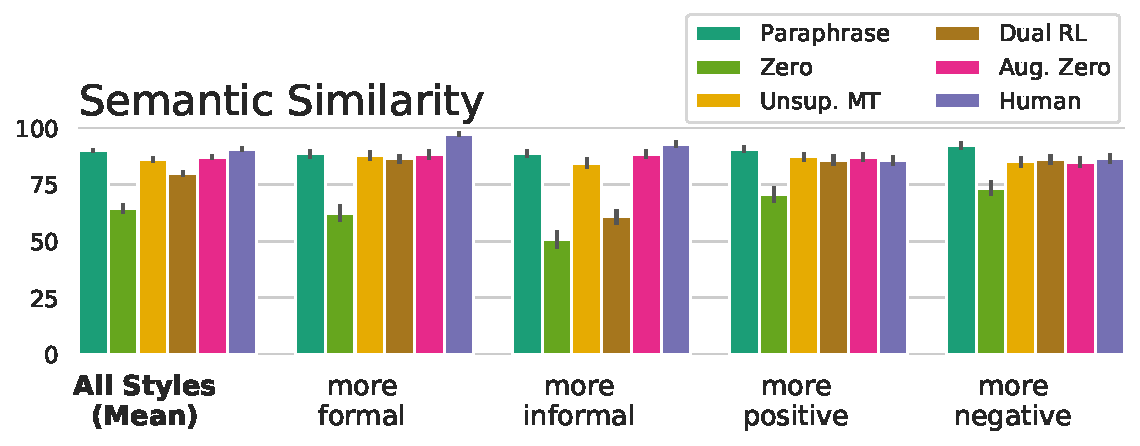
\includegraphics[width=\linewidth]{figures/meaning_standard_True.pdf}
  \caption{Human evaluation of sentiment and formality transfer. Our method is rated comparably to human-written ground truth as well as prior methods. Error bars show Standard Error of the Mean. Unsup.~MT is \citet{prabhumoye-etal-2018-style}; Dual RL is \citet{DBLP:conf/ijcai/LuoLZYCSS19}. }
  \label{human_eval_standard_style}
\end{figure}

\begin{table}[t]
\caption{
Comparing augmented zero-shot prompting with supervised style transfer methods on the Yelp sentiment style transfer dataset using automatic evaluation.
Acc: accuracy; PPL: perplexity.  The inference-only table shows our method applied to 3 different sizes of GPT-3, plus our own LLM. 
% For sentiment style transfer, we show accuracy, BLEU, and perplexity (PPL) reported as the average of positive $\rightarrow$ negative and negative $\rightarrow$ positive. 
% In (a), augmented zero-shot prompting of GLM and GPT-3 are compared with prior supervised style transfer methods.
% In (b), we compare zero-shot, five-shot, and augmented zero-shot prompting for our GLM models. 
% Candidate selection means that of the sixteen examples returned by the API, we choose the one with the highest BLEU with the source sentence (in the default case, we just use the first returned output).  
}
        \label{tab:summary_table}
    \setlength{\tabcolsep}{3pt}
    \centering \small 
        \begin{tabular}{l r r r}
        \toprule
         & Acc & BLEU & PPL\\
        \midrule
        \underline{\textsc{Supervised Methods}} \\
        Cross-alignment \citep{NIPS2017_2d2c8394} & 73.4 & 17.6 & 812 \\
        Backtrans \citep{prabhumoye-etal-2018-style} & 90.5 & 5.1 & 424 \\
        Multidecoder \citep{AAAI1817015}  & 50.3 & 27.7 & 1,703\\
        Delete-only \citep{li-etal-2018-delete} & 81.4 & 28.6 & 606 \\
        Delete-retrieve \citep{li-etal-2018-delete} & 86.2 & 31.1 & 948\\
        Unpaired RL \citep{xu-etal-2018-unpaired} & 52.2 & 37.2 & 2,750\\
        Dual RL \citep{DBLP:conf/ijcai/LuoLZYCSS19} & 85.9 & 55.1 & 982\\
        Style transformer \citep{dai-etal-2019-style} & 82.1 & 55.2 & 935\\
        \midrule
        \underline{\textsc{Inference-only methods}} \\
        GPT-3 ada, aug zero-shot& 31.5 & 39.0 & 283\\
        GPT-3 curie, aug zero-shot& 53.0 & 48.3 & 207\\
        GPT-3 da vinci, aug zero-shot& 74.1 & 43.8 & 231\\
        % \midrule
        LLM: zero-shot & 69.7 & 28.6 & 397 \\ 
        {\color{white}LLM: }five-shot & 83.2 & 19.8 & 240 \\
        {\color{white}LLM: }aug zero-shot & 79.6 & 16.1 & 173 \\
        % \midrule
        LLM-dialog: zero-shot & 59.1 & 17.6 & 138 \\
        {\color{white}LLM-dialog: }five-shot & 94.3 & 13.6 & 126 \\
        {\color{white}LLM-dialog: }aug zero-shot & 90.6 & 10.4 & 79 \\
        % \midrule
        % GLM & 65.0 & 49.3 & 292 & 10.3 \\
        % GLM-dialog & 73.7 & 40.6 & 184 & 10.7 \\
        % GLM & 79.6 & 16.1 & 173 \\
        % GLM-dialog & 90.6 & 10.4 & 79\\
        \bottomrule
        \end{tabular}
    % \vspace{3mm}
\end{table}
% \footnote{ \url{https://huggingface.co/transformers/task_summary.html#sequence-classification}} \footnote{\url{https://github.com/luofuli/DualRL}}
% , and so we automatically evaluate several aspects of our model on the Yelp sentiment classification dataset.
% Specifically, we evaluate accuracy according to a pre-trained sentiment classifier,\footnote{\url{https://huggingface.co/transformers/task_summary.html#sequence-classification}} BLEU score with respect to ground truth human examples provided by \citet{DBLP:conf/ijcai/LuoLZYCSS19},\footnote{\url{https://github.com/luofuli/DualRL}} and perplexity of generated outputs as measured by GPT-2 (117B).

Table \ref{tab:summary_table} shows these automatic evaluations, with four main takeaways. 
First, augmented zero-shot prompting achieves high accuracy and low perplexity compared with baselines. The BLEU scores, however, the outputs of our model had low BLEU scores with respect to human generated outputs \ref{tab:summary_table}. 
Based on qualitative examination of outputs, we believe that this is because our model outputs often used different language from human annotations,  despite having high semantic similarity with the source sentence.
For instance, for transferring the sentiment of ``\textit{ever since joes has changed hands it's just gotten worse and worse}'' to positive sentiment, our augmented zero-shot learning model outputted ``{the establishment has continued to provide excellent service, improving steadily since its change of ownership}.'' 
This will have low BLEU with the ground truth with respect to human references, which is simply ``\textit{ever since joes has changed hands it's just gotten better and better}.'' 
Though we do not see this as an inherent problem, increasing the BLEU for the purposes of comparison can be done in an easy way via candidate selection, as our model returns sixteen possible continuations. In applications for which we prefer model outputs to have high lexical similarity to the source sentence, we could select the candidate of the sixteen with the highest BLEU score compared with the original source sentence. 
We find that this candidate selection step can substantially improve the BLEU score with the ground truth target sentences, as we show in Table \ref{tab:candidate_select}. 

\begin{table}
\caption{
Sentiment style transfer results with candidate selection (cand.~select.). 
Candidate selection means that of the sixteen examples returned by our model, we chose the one with the highest BLEU with the source sentence.  
}
\label{tab:candidate_select}
    % \setlength{\tabcolsep}{2pt}
    \centering \small 
        \begin{tabular}{l r r r}
        \toprule
         & Acc & BLEU & PPL\\
        \midrule
        \underline{LLM-128B} \\
        Zero-shot & 69.7 & 28.6 & 397 \\
        + cand.~select. & 31.4 & 61.5 & 354\\
        Five-shot & 83.2 & 19.8 & 240\\
        + cand.~select. & 61.5 & 55.6 & 306\\
        Augmented zero-shot & 79.6 & 16.1 & 173\\
        + cand.~select. & 65.0 & 49.3 & 292\\
        \midrule
        \underline{LLM-128B-dialog} \\
        Zero-shot & 59.1 & 17.6 & 138\\
        + cand.~select. & 46.8 & 24.2 & 166\\
        Five-shot & 94.3 & 13.6 & 126\\
        + cand.~select. & 81.3 & 47.6 & 345\\
        Augmented zero-shot & 90.6 & 10.4 & 79\\
        + cand.~select. & 73.7 & 40.6 & 184\\
        \bottomrule
        \end{tabular}
    % \vspace{3mm}
\end{table}



Second, we apply augmented zero-shot learning to GPT-3 175B; these results indicate that augmented zero-shot learning generalizes to another large language model.
% \footnote{GPT-3 generations were done using nucleus sampling with $p=0.6$ while LLM generation was done with top-$k$=40. This means their numbers should not be directly compared.}
Third, we vary model size for GPT-3 models, finding that larger size greatly improves style transfer. 
Fourth, for \textit{LLM} and \textit{LLM-dialog}, we find that augmented zero-shot learning substantially outperforms vanilla zero-shot learning and almost reaches the accuracy of five-shot learning. 

% As described above, we also compared performance to prior methods, on formality and sentiment. We evaluated these outputs using the same human evaluation framework described above, comparing to the same baselines (human, zero, and paraphrase), as well as two prior methods that scored highly on the automatic metrics below, \citet{prabhumoye-etal-2018-style} and \citet{DBLP:conf/ijcai/LuoLZYCSS19}. 
% Figure \ref{human_eval_form_sent} shows the results. As with the wide range of styles, the results from augmented zero shot learning were rated comparably to human generated responses on all axes, and were also in the same range of \citet{DBLP:conf/ijcai/LuoLZYCSS19}.

\subsubsection{Comparison with a range of prior methods}
To compare against a larger range of prior supervised methods, we used automatic evaluation, and found comparable performance with the highest-scoring method for transfer strength.
The results are shown in Table \ref{tab:prior-methods}.
We were also significantly more fluent than all other methods.
% However, this is hardly surprising and should be taken with a grain of salt: GPT-2 is another generative language model, so it stands to reason that the token probabilities would be similar to our model's.
Finally, our method fell short on semantic preservation compared to other methods. However, BLEU is known to penalize long sentences, and the scores do not always align with human judgements.
For example, our model's worse performance could be because it was not explicitly trained on Yelp data, so its generations are less likely to be in the style of Yelp reviews than models that were.


% \begin{table}
%     \setlength{\tabcolsep}{2pt}
%     \centering \small 
%     \begin{tabular}{l r r r r}
%     \toprule
%      & Acc & BLEU & PPL & $l$\\
%     \midrule
%     Cross-alignment \citep{NIPS2017_2d2c8394} & 73.4 & 17.6 & 812 & 10.7 \\
%     Backtrans \citep{prabhumoye-etal-2018-style} & 90.5 & 5.1 & 424 & 9.7 \\
%     Multidecoder \citep{AAAI1817015}  & 50.3 & 27.7 & 1,703 & 10.4 \\
%     Delete-only \citep{li-etal-2018-delete} & 81.4 & 28.6 & 606 & 12.1 \\
%     Delete-retrieve \citep{li-etal-2018-delete} & 86.2 & 31.1 & 948 & 11.7 \\
%     Unpaired RL \citep{xu-etal-2018-unpaired} & 52.2 & 37.2 & 2,750 & 9.4 \\
%     Dual RL \citep{DBLP:conf/ijcai/LuoLZYCSS19} & 85.9 & 55.1 & 982 & 10.1 \\
%     Style transformer \citep{dai-etal-2019-style} & 82.1 & 55.2 & 935 & 10.3 \\
%     \midrule
%     \underline{Augmented Zero-Shot Prompting} \\
%     GPT-3 ada & 31.5 & 39.0 & 283 & 10.0 \\
%     GPT-3 curie  & 53.0 & 48.3 & 207 & 10.3 \\
%     GPT-3 da vinci  & 74.1 & 43.8 & 231 & 10.4 \\
%     \midrule
%     GLM & 65.0 & 49.3 & 292 & 10.3 \\
%     GLM-dialog & 73.7 & 40.6 & 184 & 10.7 \\
%     \bottomrule
%     \end{tabular}
%     \vspace{3mm}
%   \caption{
%           For sentiment style transfer, we show accuracy, BLEU, perplexity (PPL), and sequence length ($l$) for augmented zero-shot prompting compared with prior supervised style transfer methods.
%           Results shown are the average of positive $\rightarrow$ negative and negative $\rightarrow$ positive. 
%   \label{tab:prior-methods}
%   }
% \end{table}
% % \end{wraptable}



\begin{table}
    \setlength{\tabcolsep}{2pt}
    \begin{subtable}{.58\linewidth}
    \centering \small 
        \begin{tabular}{l r r r r}
        \toprule
         & Acc & BLEU & PPL & $l$\\
        \midrule
        Cross-alignment \citep{NIPS2017_2d2c8394} & 73.4 & 17.6 & 812 & 10.7 \\
        Backtrans \citep{prabhumoye-etal-2018-style} & 90.5 & 5.1 & 424 & 9.7 \\
        Multidecoder \citep{AAAI1817015}  & 50.3 & 27.7 & 1,703 & 10.4 \\
        Delete-only \citep{li-etal-2018-delete} & 81.4 & 28.6 & 606 & 12.1 \\
        Delete-retrieve \citep{li-etal-2018-delete} & 86.2 & 31.1 & 948 & 11.7 \\
        Unpaired RL \citep{xu-etal-2018-unpaired} & 52.2 & 37.2 & 2,750 & 9.4 \\
        Dual RL \citep{DBLP:conf/ijcai/LuoLZYCSS19} & 85.9 & 55.1 & 982 & 10.1 \\
        Style transformer \citep{dai-etal-2019-style} & 82.1 & 55.2 & 935 & 10.3 \\
        \midrule
        \underline{Augmented Zero-Shot Prompting} \\
        GPT-3 ada & 31.5 & 39.0 & 283 & 10.0 \\
        GPT-3 curie  & 53.0 & 48.3 & 207 & 10.3 \\
        GPT-3 da vinci  & 74.1 & 43.8 & 231 & 10.4 \\
        \midrule
        % GLM & 65.0 & 49.3 & 292 & 10.3 \\
        % GLM-dialog & 73.7 & 40.6 & 184 & 10.7 \\
        % GLM & 65.0 & 49.3 & 292 & 10.3 \\
        % GLM-dialog & 90.6 & 10.4 & 79 & 10.7 \\
        \bottomrule
        \end{tabular}
        \label{tab:prior-methods}
        \caption{}
    \end{subtable}
    \begin{subtable}{.40\linewidth}
    \centering \small 
        \begin{tabular}{l r r r r}
        \toprule
         & Acc & BLEU & PPL & $l$\\
        \midrule
        \underline{GLM} \\
        Zero-shot & 69.7 & 28.6 & 397 & 9.6 \\
        + cand.~selection & 31.4 & 61.5 & 354 & 10.2 \\
        Five-shot & 83.2 & 19.8 & 240 & 11.2 \\
        + cand.~selection & 61.5 & 55.6 & 306 & 10.2 \\
        Augmented zero-shot & 79.6 & 16.1 & 173 & 11.3 \\
        + cand.~selection & 65.0 & 49.3 & 292 & 10.3 \\
        \midrule
        \underline{GLM-dialog} \\
        Zero-shot & 59.1 & 17.6 & 138 & 17.2 \\
        + cand.~selection & 46.8 & 24.2 & 166 & 17.2  \\
        Five-shot & 94.3 & 13.6 & 126 & 13.3 \\
        + cand.~selection & 81.3 & 47.6 & 345 & 10.0 \\
        \textbf{Augmented zero-shot} & \textbf{90.6} & \textbf{10.4} & \textbf{79} & 12.8 \\
        + cand.~selection & 73.7 & 40.6 & 184 & 10.7 \\
        \bottomrule
        \end{tabular}
        \caption{}
        \label{tab:ablation}
    \end{subtable}
    \vspace{3mm}
\caption{
For sentiment style transfer, we show accuracy, BLEU, perplexity (PPL), and sequence length ($l$) reported as the average of positive $\rightarrow$ negative and negative $\rightarrow$ positive. 
In (a), augmented zero-shot prompting of GLM and GPT-3 are compared with prior supervised style transfer methods.
In (b), we compare zero-shot, five-shot, and augmented zero-shot prompting for our GLM models. 
Candidate selection means that of the sixteen examples returned by the API, we choose the one with the highest BLEU with the source sentence (in the default case, we just use the first returned output).  
}
\end{table}
% \end{wraptable}

\subsubsection{Comparison across Different LLMs}
We also compared between three varieties of model: GPT-3 \citep{DBLP:journals/corr/abs-2005-14165}, LLM, and  LLM-Dialog. We adjusted the prompt template slightly to accommodate these differences: for  LLM and GPT-3, the prompt template replaced {\small
\texttt{``Rewrite it to be \textbf{<style>}''}
with \small \texttt{``Here is a rewrite of the text, which is \textbf{<style>}''}.}
For our augmented zero-shot prompts we also see that the LLM-dialog version had higher accuracy than the LLM and GPT-3, but lower BLEU. Based on qualitative inspection, we believe the lower BLEU is due to the LLM-dialog adding additional detail in the generated sentences, which is consistent with an ``interestingness'' objective that is typically encoded into dialog training. 


\subsubsection{Prompt Construction}
\label{sec:prompt-selection}
Prompt engineering can be brittle: \citet{reynolds2021prompt} describe how reformulating the language of a prompt can have significant impact on performance, and that finding the right prompt is for a task is more akin to locating an already-learned task than truly learning a new one.
To explore this, we compared several variations of the prompts for sentiment, varying the language of the prompt to use ``\textit{more {positive/negative}},'' ``\textit{{happier/sadder}},''
``\textit{more {optimistic/pessimistic}},'' or
``\textit{more {cheerful/miserable}}.''
As shown in Table~\ref{tab:compare-between-prompts}, performance differed across the four prompts, but we found them comparable.
In a real world setting, our augmented zero-shot approach allows users to effortlessly try out many different phrasings for the task until they find one that performs satisfactorily.

\begin{table}[ht]
    \centering \small 
    \begin{tabular}{lrrr}
    \toprule
    Model / prompt wording &Acc&Bleu&PPL \\
    \midrule
    \underline{LLM}&&&\\
    ``more {positive/negative}''&76.3&14.8&180\\
    ``{happier/sadder}''&62.6&15.5&173\\
    ``more {optimistic/pessimistic}''&69.7&14.1&143\\
    ``more {cheerful/miserable}''&74.5&15.7&186\\
    \midrule
    \underline{LLM-Dialog}&&&\\
    ``more {positive/negative}''&90.5&10.4&79 \\
    ``{happier/sadder}''&85.9&9.6&90 \\
    ``more {optimistic/pessimistic}''&85.8&10.2&79 \\
    ``more {cheerful/miserable}''&88.8&11.4&93 \\
    \bottomrule
    \end{tabular}
\caption{Comparing variations of augmented zero-shot learning prompt wording for sentiment style transfer.}
\label{tab:compare-between-prompts}
\end{table}

\citet{reynolds2021prompt} further emphasize that prompt engineering is mostly about avoiding various failure cases.
 In this work, we use delimiters (``\{'' and ``\}'') to help avoid parsing errors, giving scores of zero when there was no valid responses with such delimiters. There are other delimiters that could be used (e.g., quotes, ``('' and ``)'', ``<'' and ``>'', newlines with a colon (as used by GPT-3), etc. We chose curly braces as they were 1) likely to occur in the training data as delimiters in other contexts and 2) not frequently part of the input sentence itself. We also use a second person prompt template for the dialog, which yielded better results as it was more similar to the training data. Exploring these options more quantitatively would be an interesting direction for future work.


\subsection{Potential of Arbitrary Styles}\label{subsec:potential}
 
\begin{table}[t]
\caption{\label{tab:unique_requests}Requests in the form of ``\textit{Rewrite this...}'' made by real users to a large LM-powered text editor.}
\label{tab:realusers}
\small
% \resizebox{\columnwidth}{!}{%
\def\arraystretch{1.5}% 
\begin{tabular}{p{1.0\columnwidth}}
% \textbf{Rewrite requests (user completions of `Rewrite this...')} \\
\midrule
into paragraphs • to be a bit clearer • to be a little less angsty • to be a word for a song • to be about mining • to be about vegetables • to be better written • to be less descriptive • to be less diabolical • to be more absurd • to be more adventurous • to be more angry • to be more cheerful • to be more descriptive • to be more Dickensian • to be more emotional • to be more fancy • to be more flowery • to be more interesting • to be more joyful • to be more magical • to be more melodramatic • to be more philosophical • to be more revolutionary • to be more scary • to be more subtle • to be more surprising • to be more suspenseful • to be more technical • to be more violent • to be more whimsical • to be warmer • to fit better grammatically with the rest of the story • to make more sense • to use a more interesting word • with a few words \\
\midrule
\end{tabular}
% }
% \vspace*{3mm}
\end{table}

% The adaptability of our method to arbitrary styles is compelling because it facilitate an AI-powered writing assistant that transforms text to any desired re-write specified by a user. 
One promising application of augmented zero-shot learning is an AI-powered writing assistant that can allow writers to transform their text in arbitrary ways that the writer defines and controls.
As a qualitative case study to explore what arbitrary re-write styles may be requested, we built an AI-assisted story-writing editor with a ``rewrite as'' feature that uses our augmented few-shot method.
Our editor has a freeform text box for users to specify how they would like a selection of their story to be rewritten (Figure \ref{fig:wc}).
% We asked 30 fluent English speakers from a creative writing group to write a 100-300 word story based on a prompt.
We asked 30 people from a creative writing group to use our UI to write a 100-300 word story,  collecting 333 rewrite requests in total. 
Table \ref{tab:unique_requests} shows a list of unique rewrite requests collected from 30 early users recruited from a creative writing mailing list.
These were as diverse as asking for the text ``\textit{to be about mining}'' or ``\textit{to be less diabolical}.''
Overall, we collected 333 rewrite requests, of which users chose to insert the model's response into their story 18 (5.4\%) times.


\subsection{Limitations and Failure Modes}
\label{section:limitations}
This section details several qualitative limitations with our method.
\subsubsection{Unparsable answers} A frequent problem that arises when using large LMs for other NLP tasks is their outputs cannot be automatically parsed into usable answers. For example, when given a prompt like \begin{small}
 \texttt{``Here is some text: {that is an ugly dress}. Here is a rewrite of the text, which is more positive''} \end{small}
 \textit{LLM-Dialog} might return something like \begin{small}
 \texttt{``Sounds like you are a great writer!''} \end{small} Similar error modes exist for \textit{LLM}, which might output something like \begin{small}
 \texttt{``Here are more writing tips and tricks.''} \end{small} Other times, the response contains correct information, but it cannot be automatically parsed (e.g., \begin{small}
 \texttt{``a good rewrite might be to say that the dress is pretty.''} \end{small}) In hindsight, these outputs make a lot of sense: most of the training data of large LMs is not well-formatted pairs of inputs and outputs  \citep{reynolds2021prompt}. See $\S$\ref{sec:prompt-selection} for how we dealt with these issues.

\subsubsection{Hallucinations} Large LMs are known to hallucinate text content; we saw this happen frequently for style transfer. While this is an advantage in some contexts like creative writing, it is undesirable for applications like summarization. 
% Other prior methods, such as those based on word replacement, do much better at keeping the meaning and format of the sentence the same.
% \citep{DBLP:journals/corr/abs-2010-03802} have even explored the ability to ``tune in'' the amount of style-- a future direction for our work would be to explore this as well.
\subsubsection{Inherent style trends} We also noticed that even our \textit{``paraphrase''} baseline, where the model was simply asked to rewrite the input sentence, was rated highly for style strength for a few styles, including \textit{``more formal''} and \textit{``more melodramatic''}.
This implies that our method's generations generally trend toward these styles.
A direction for future work would be to see what styles and qualities of text our method (and large LMs in general) are inherently more likely to produce.

\subsubsection{Less reliable than trained methods}
For style transfer tasks that have available training data, prior methods that either train or finetune on that data are going to be inherently more reliable at producing text that looks like their training data.
This can be observed in the lower BLEU scores our method achieves than trained methods, despite comparable transfer accuracy.
Thus, augmented zero-shot learning offers less fine-grained controllability in the properties of the style-transferred text than methods which see task-specific training data.

\subsubsection{Large LM safety concerns} Large LMs themselves come with their own host of difficulties, barriers to entry, and potential safety concerns as discussed by \citet{bender2021stochastic}, which are also valid for this style transfer method. However, we also think that this method can be a useful tool in exploring and exposing the safety and boundaries of these models themselves: what happens if we try to force the large LM to make a text ``more racist'', ``more sexist'', or ``more incendiary''? It is important to keep pushing these models to their boundaries to see where they fail and where problems arise, and specific use cases that show a broader range of the model's capabilities also show a broader range of its failure modes.


\begin{table}[ht]
    \caption{Examples of users' arbitrary style transfer requests for which the model suggestion was accepted.}
    \label{tab:selected_usage_examples}
    \small
    \centering
    \def\arraystretch{1.5}% 
    \begin{tabular}{p{0.41\linewidth} p{0.45\linewidth}}
    \toprule
      \textbf{Input} & \textbf{Model suggestion} \\ \midrule
      You honor me,'' said Bruno. As he spoke, he began to laugh. His laugh was merry sounding and melodic. He took a deep breath. When he spoke again, his voice was low and strong. ``I take this great task on and with my brothers shall lead us on to victory! \newline \textbf{Rewrite it to be about mining.} & You honor me, said Bruno. As he spoke, he began to laugh. His laugh was deep and gravely, as if from the bowels of the earth. He took a deep breath. When he spoke again, his voice was deep and dark.`I take this great task on and with my brothers shall delve into the mines!'' \\ \midrule
      I reckon,' smiled Toe, 'you'd have to say the same for icicles, wouldn't you? \newline \textbf{Rewrite it to be more interesting.} & ‘I reckon,’ smiled Toe, ‘you’d have to say the same for icicles, wouldn’t you?’ These words were barely out of his mouth before the others realized exactly what they meant.\\ \midrule
      with its southern perfume \newline \textbf{Rewrite it to be more descriptive} & A mixture of sweet honeysuckles and jasmine  with  a  hint  of  tobacco  and warm mesquite smoke. It was his southern perfume, with a hint of a memory of simpler times.\\ \midrule
      But Sally remained unmoved--and lonely. \newline \textbf{Rewrite it to be more emotional} & Her tears rolled and rolled down her cheek, mixing with the saltwater around her, until the water was a rich mixture of the two. She wanted her poem to be cheerful like it used to be, but couldn't find the right words. \\
    \bottomrule
    \end{tabular}
\end{table}

\begin{table}[ht]
    \caption{In black, we show the exact augmented-zero shot prompts used in our experiments, for \textit{LLM} and GPT-3 (top), and for \textit{LLM-Dialog} (bottom). As shown, for \textit{LLM-Dialog}, we replaced ``\texttt{Here is a rewrite of the text, which is}'' with ``\texttt{Rewrite it to be}''. Each line starting with ``>"" above was passed in as an individual dialog turn. 
    The blue shows how an input text and goal style are concatenated to the few-shot prompt in order to produce final model output.
    Note that we can achieve high accuracy even though the prompt formulation resulted in some minor grammatical errors for some styles (e.g., ``\texttt{rewrite it to be include the word 'snow'}''). Text versions of these prompts can be downloaded at \url{https://bit.ly/3fLDuci}.}
    \label{tab:fullprompt}
    \centering
    \tiny
    \begin{tabular}{p{.9\linewidth}}
\midrule
\multicolumn{1}{c}{Augmented Zero-shot Prompt: LLM}
\\
\texttt{Here is some text: \{When the doctor asked Linda to take the medicine, he smiled and gave her a lollipop.\}. Here is a rewrite of the text, which is more scary. \{When the doctor told Linda to take the medicine, there had been a malicious gleam in her eye that Linda didn't like at all.\} Here is some text: \{they asked loudly, over the sound of the train.\}. Here is a rewrite of the text, which is more intense. \{they yelled aggressively, over the clanging of the train.\} Here is some text: \{When Mohammed left the theatre, it was already dark out\}. Here is a rewrite of the text, which is more about the movie itself. \{The movie was longer than Mohammed had expected, and despite the excellent ratings he was a bit disappointed when he left the theatre.\} Here is some text: \{next to the path\}. Here is a rewrite of the text, which is about France. \{next to la Siene\} Here is some text: \{The man stood outside the grocery store, ringing the bell.\}. Here is a rewrite of the text, which is about clowns. \{The man stood outside the circus, holding a bunch of balloons.\} Here is some text: \{the bell ringing\}. Here is a rewrite of the text, which is more flowery. \{the peales of the jangling bell\} Here is some text: \{against the tree\}. Here is a rewrite of the text, which is include the word "snow". \{against the snow-covered bark of the tree\}} 
\textcolor{blue}{\texttt{Here is some text: \{That is an ugly dress\}. Here is a rewrite of the text, which is more positive."}}
\\
\midrule
\multicolumn{1}{c}{Augmented Zero-shot Prompt: LLM-dialog}
\\
\texttt{> Here is some text: \{When the doctor asked Linda to take the medicine, he smiled and gave her a lollipop.\}. Rewrite it to be more scary. \newline
> \{When the doctor told Linda to take the medicine, there had been a malicious gleam in her eye that Linda didn't like at all.\} \newline
> Here is some text: \{they asked loudly, over the sound of the train.\}. Rewrite it to be more intense. \newline
> \{they yelled aggressively, over the clanging of the train.\} \newline
> Here is some text: \{When Mohammed left the theatre, it was already dark out\}. Rewrite it to be more about the movie itself. \newline
> \{The movie was longer than Mohammed had expected, and despite the excellent ratings he was a bit disappointed when he left the theatre.\} \newline
> Here is some text: \{next to the path\}. Rewrite it to be about France. \newline
> \{next to la Siene\} \newline
> Here is some text: \{The man stood outside the grocery store, ringing the bell.\}. Rewrite it to be about clowns. \newline
> \{The man stood outside the circus, holding a bunch of balloons.\} \newline
> Here is some text: \{the bell ringing\}. Rewrite it to be more flowery. \newline
> \{the peals of the jangling bell\} \newline
> Here is some text: \{against the tree\}. Rewrite it to be include the word "snow". \newline
> \{against the snow-covered bark of the tree\} \newline
}
\textcolor{blue}{\texttt{> Here is some text: \{That is an ugly dress\}. Rewrite it to be more positive."}}
\\
\midrule
\end{tabular}
\end{table}

\begin{figure}[!htb]
  \centering
  \fbox{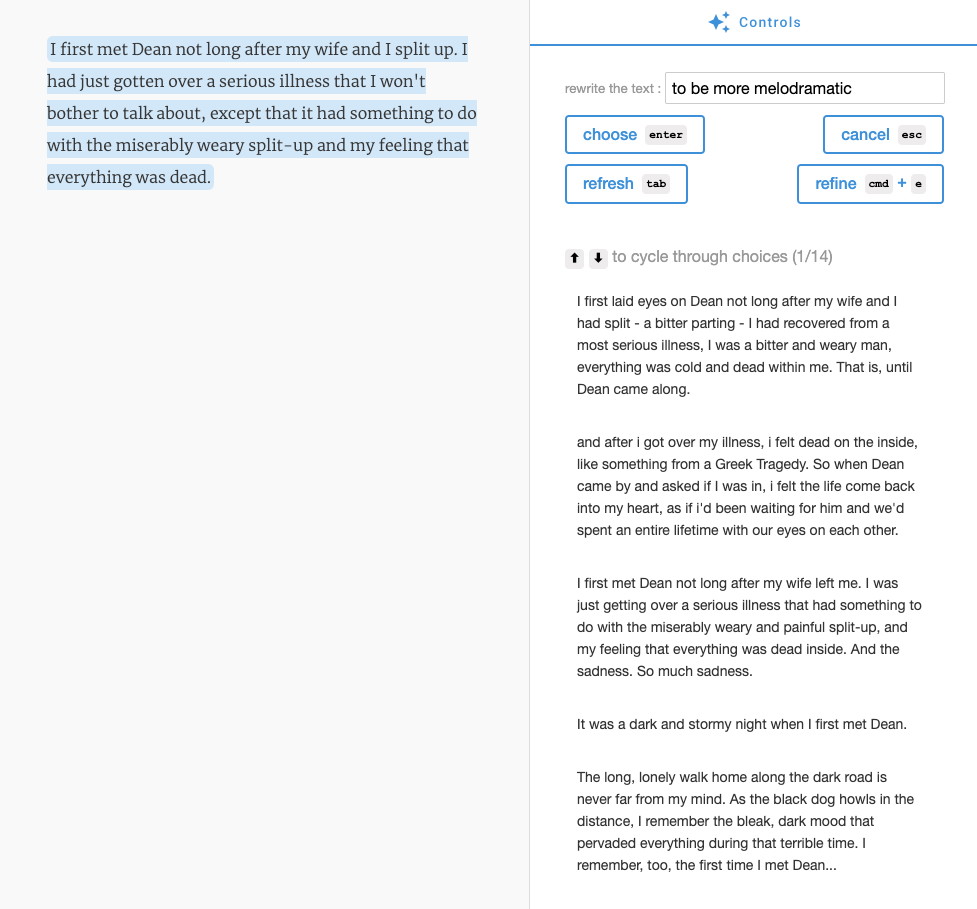
\includegraphics[width=1\linewidth]{figures/wc.png}}
  \caption{Screenshot AI-assisted editor with `Rewrite as' feature.\label{fig:wc}}
  \vspace{-0.1cm}
\end{figure} 

\subsection{Summary of Contributions}
The work described in this section was published in the 2022 Proceedings of the Association of Computational Linguistics \TODO{citation}.
The work was performed with my collaborators \TODO{author names}.
I worked with Emily Reif to come up with the premise for the project: of formulating style transfer as an arbitrary rewriting operation.
I helped to design the experiments and contributed significantly to analysis of the results.


\section{Wordcraft: An editor for AI-assisted writing.}
\label{section:wordcraft}

How do we evaluate natural language generation in realistic settings? In all the human evaluations discused so far in my thesis, we recruited annotators to evaluate text in artifical settings. In Sections \ref{section:detection} and \ref{section:roft}, university students were asked to label text as human-written or machine-generated in user interfaces custom-tailored to collect these sorts of annotations. In Sections \ref{section:fitb} and Section \ref{section:style_transfer}, novel natural language systems were evaluated by asking raters on Amazon Mechnical Turk to view and score generated text.
Notably, the annotators were not asked to use the proposed NLG tools to accomplish a task of interest; they were only asked to evaluate pre-generated outputs.

When building novel systems for cotrollable text generation, it is crucial to keep in mind why these tools are being built and who their target audience might be.
This is especially true in the area of AI-assisted creative writing, where there is often significant discrepency between how novel tools are evaluated (Amazon Mechanical Turker workers paid per annotation) and how they are intended to be used in the real world (writers seeking support or inspiration while performing their craft).

Wordcraft is an AI-augmented text processor which is intended as a real-world test bed for controllable text generation paradigms in the domain of creative writing.
Our goal in developing Wordcraft was to learn how people interact with modern state-of-the-art NLG systems, what tasks they ask the NLG systems to do do and how well the systems deliver, and how this feeds back into the works people ultimately create.
The user interface for Wordcraft consists of of a traditional text editor alongside a set of controls that vary based on where the user's cursor is and whether they have selected any text.
The user also has access to a chatbot they can talk about their story with.

In this section, I describe the controls included in  Wordcraft, how they're implemented, and the motivation for including them.
I then describe how Wordcraft offers the chance for a more realistic evaluation of state-of-the-art language generation systems through user studies with both amateur and expert writers.


\subsection{Features of Wordcraft}
\label{section:wordcraft_controls}
Wordcraft uses few-shot in-context learning techniques \cite{brown2020language} to support a variety of generative controls.
The underlying neural language model backing all these interactions is LaMDA \cite{thoppilan2022lamda}, which is described in detail in Section \ref{subsection:lambda_description}.
Because LaMDA was finetuned for dialog, we frame our prompts in terms of a conversation.
The remainder of this section enumerates the controls available in Wordcraft and gives an example few-shot prompt that supports each.
In practice, the examples used in the few-shot prompt are randomly sampled from a small pool of examples each time the user selects a control.
Each control in Worcaft results in several candidate generations being presented to the user.
When a generation is selected by the user, it is inserted into the text at the location of the user's cursor.


\subsubsection{Continuation}
As described in Section \ref{section:background_gen}, continuation is the default action of a left-to-right neural language model such as LaMDA, achieved simply by prompting the LM with a text passage, and decoding a possible continuation.
A continuation generator is useful to writers who want text appended to the end of what they have written so far.
This control is available when the user's cursor is at the end of the text passage.

\subsubsection{Initial Story Ideas}
When the user has no text inputted, the user can specify the topic they want their story to be about and then have Wordrcraft generate starting sentences.
The intention of this control is to allow for ideation when the page is blank.
It is supported with the following few-shot prompt:

\begin{verbatim}
> Here's a topic: {A space monkey needs to escape from his dying planet.} Tell me the start of a new story.
> {It was a cold, dark night on an unknown planet. In a field, a male monkey was pacing back and forth. He had been trying to figure something out, but nothing seemed to be working. He didn't have much time left.}
> Here's a topic: {A medieval romance where a group of colorful knights do battle.} Tell me the start of a new story.
> {The green knight rode atop his majestic, beautiful horse, across fields of pure green. In his palm was a magical, sparkling golden sword.}
> Here's a topic: {An old man with a magical box tries to solve a mystery as his memories gradually fade away.} Tell me the start of a new story.
> {The old man decided that he should look inside the box, and in the box there was a key. The old man couldn’t quite remember why he had a key, but he knew the key was important.}
> Here's a topic: {A coven of witches have taken up residence outside of a quiet mountain town, but they're not interested in witchcraft, they're interested in making hip-hop.} Tell me the start of a new story.
> {An evil looking tree was growing off in the distance with no leaves and long, pointy branches. It was a sickly green and was swaying eerily without the wind.}
> Here's a topic: {After an ancient sea-worn bottle washes up on the shores of Tripoli, a group of rag-tag pirates open it up to find a map leading to a magical treasure.} Tell me the start of a new story.
> {A group of pirates set out to sea in search of a magical treasure - a long, sparkling blue necklace called the night's eye.}
> Here's a topic: {<USER'S TOPIC>} Tell me the start of a new story.}
\end{verbatim}
% This is based on the arbitrary style transfer technique described in Section \ref{section:style_transfer}.

\subsubsection{Fill in the blank}
When the user has some text selected in the editor, they are able to see alternatives that fit into the place of their selection.
This is exactly the fill-in-the-blank task described in Section \ref{section:fitb}.
Though in Section \ref{section:fitb} we showed that finetuned models perform much better at this than few-shot prompting techniques, due to the computational complexities of hosting multiple models, we ended up also supporting this operation with a few-shot learning prompt:

\begin{verbatim}
> {\"We have to leave now!\" Sarah shouted.  ____ The only way out was up. We climbed flight after flight. The sound of the monsters banging on the door below became more distant but no less threatening.} Finish the following sentence by filling in the blank with a phrase. {\"We have to leave now!\" Sarah shouted.  }
> {\"Let's get out of here!\"}
> Here's a new story: {The sun was shining, and little gusts of wind brought through the window  ____ shocking contrast from the stale city smells she had grown used to.} Finish the following sentence by filling in the blank with a phrase. {The sun was shining, and little gusts of wind brought through the window  ____ shocking contrast from the stale city smells she had grown used to.}
> {the faint scent of huneysuckle. It was a}
> Here's a new story: {I was minding my business at the park, when I was approached by a little girl who was crying because she had lost  ____ so of course I helped search.} Finish the following sentence by filling in the blank with a phrase. {I was minding my business at the park, when I was approached by a little girl who was crying because she had lost  ____ so of course I helped search.}
> {her new kitten.}
> Here's a new story: {It was a cold night, and a storm was raging out at sea. A lightning bolt lit up the sky, briefly illuminating the lighthouse  ____ plummeted but just before reaching the churning water, he disappeared in a poof of purple flame!} Finish the following sentence by filling in the blank with a phrase. {A lightning bolt lit up the sky, briefly illuminating the lighthouse  ____ plummeted but just before reaching the churning water, he disappeared in a poof of purple flame!}
> {in a sharp silhouette.}
> Here's a new story: {The magician pulled out of his pocket  ____  and then a second one and a third. He didn't stop until soon the ground was covered with them.} Finish the following sentence by filling in the blank with a phrase. {The magician pulled out of his pocket  ____  and then a second one and a third. }
> {a scarlet handkerchief }
> Here's a new story: {<USER'S STORY>} Finish the following sentence by filling in the blank with a phrase. {<USER'S SELECTED SENTENCE WITH BLANK AT POSITON OF CURSOR>}
\end{verbatim}

\subsubsection{Elaboration}
When the user has some text selected, they can use the elaboration button to get the model to expand upon it.
This operation is supported with the following few-shot prompt:

\begin{verbatim}
Here's a new story: {The long shadow of the tree crept up the sidewalk} Describe the tree.
{It was an old oak tree on the main street of a small town, the branches spread as large as the sky.}
Here's a new story: {The car came bouncing down the hill and came to an abrupt stop in my driveway} Describe the car.
{It was an old, old Model-T Ford, with brass fittings, and no doors}
Here's a new story: {My pencil sits on top of the desk, left there since ‌the events‌ of last Saturday} Describe last Saturday.
{It was one of those Saturdays that starts off like any other but you have the feeling that something is about to stir. You wake up with the same amount of enthusiasm but you get up from bed a little slower than usual. You know this is going to be a busy day}
Here's a new story: {She wasn't really upset about what had happened at the lab the other day; she was never one to dwell on mistakes.} Describe what had happened.
{She had accidentally left the microorganisms alone for far too long. The lab, or what was left of it, was now filled with a strong aroma of their slime-- they had devoured all the metal, wood, and plastic they could find}
Here's a new story: {<USER'S STORY>} Describe \textbf{<USER'S SELECTED TEXT>}.
\end{verbatim}

\subsubsection{Style Transfer}
Using the augmented zero-shot learning approach described in Section \ref{section:style_transfer}, we include a control that allows users to perform rewriting operations on selected text. The operations are specified in natural language.
The following prompt is used.

\begin{verbatim}
> Here's a new story: {An elderly man was sitting alone on a dark path. The darkness turned to light as a figure ran up to him. ____ The older man recognized the young man as a dear friend, who he hadn't seen in some time. The young man said he had had the strangest dream.} What sentence goes in the blank?
> {The figure was holding a sword.}
> Rewrite the sentence to use more descriptive language.
> {The shadowy figure held in his hand a shining sword that glimmered in the darkness.}
> Here's a new story: {There once was a man named Kentucky, who could play the guitar like nobody's business.____Kentucky was a lonely man living in a lonely house in the middle of nowhere with only his favorite guitar to keep him company. Now this guitar had been owned by many-a-man, and all of them had come to the same fate. They played the guitar until the guitar played them.} What sentence goes in the blank?
> {He loved to play the guitar so that he could hear the guitar sing along to him, to hear the guitar's melodic hum.}
> Rewrite the sentence to be more melancholy.
> {He loved playing sad songs on his weathered guitar, so he could drown out his loneliness with the guitar's melodic hum.}
> Here's a new story: {A small group of explorers landed in China, and were amazed by the beautiful, sparkling buildings. They wondered how such a beautiful country could ever be as scary as they had heard. It was at night, and the explorers were deep in the heart of the forbidden city, their flashlights not strong enough to reach the bottom of the narrow, dark hallways.____} What sentence goes in the blank?
> {Suddenly, a terrifying sound echoed through the halls.}
> Rewrite the sentence to use more interesting words.
> {Out of nowhere, a thunderous cacophony reverberated through the halls.}
> Here's a new story: {An elderly man was sitting alone on a dark path. ____ It was a plain pine box and looked as if it had been there for a long time. The man was afraid to look inside the box.} What sentence goes in the blank?
> {The man looked down at his feet, and realized he was standing next to a box.}
> Rewrite the sentence to be more evocative.
> {The man nearly gasped as he peered down at his feet, suddenly realizing he was standing next to a mysterious box.}
> Here's a new story: {Once upon a time, there was a rabbit princess. The bunny lives in the little cottage just outside of town. The story ends with her getting eaten by a fox. ____ The door hung at an angle off of its hinges.} What sentence goes in the blank?
> {<SELECTED TEXT>}
> Rewrite the sentence <REWRITING INSTRUCTION>.
\end{verbatim}

\subsubsection{Custom Prompting}
In the custom prompting control, users have the ability to write any request to the system they want. For example, they could ask "Give me an origin story for the ogre" or "Tell me what happens next." We use a similar approach to style transfer, with a prompt demonstrating a variety of requests:

\begin{verbatim}
> Here is some text: {next to the path} Rewrite it to be about France.
> {next to la Siene}
> Here's a new story: {A young boy was sitting on the sidewalk.} What comes next?
> {He was holding a lantern and looking ahead up the road.‌}
> Here is some text: {The man stood outside the grocery store, ringing the bell.} Rewrite it to be about clowns.
> {The man stood outside the circus, holding a bunch of balloons.}
> Here's a new story: {My pencil sits on top of the desk, left there since ‌the events‌ of last Saturday.} Describe last Saturday.
> {It was one of those Saturdays that starts off like any other but you have the feeling that something is about to stir. You wake up with the same amount of enthusiasm but you get up from bed a little slower than usual. You know this is going to be a busy day}
> Here's a new story: {<USER'S STORY>} <CUSTOM PROMPT>
\end{verbatim}

\subsection {Suggested Prompts}
Finally, we implemented a control that allows users to request suggestions for what to write about next.
We expected this feature to be useful for novice writers to overcome writer's block.
It uses the following prompt:

\begin{verbatim}
> Here's a new story: {A long time ago, in the beginning of time, beautiful crystalline frog people inhabited the earth. Their king, the crystal king, had mysteriously disappeared on a trip to the sea.} What would you tell me about next?
> {Tell me more about the frog people.}
> Here's a new story: {The green knight rode atop his majestic, beautiful horse, across fields of pure green. In his palm was a magical, sparkling golden sword.} What would you tell me about next?
> {Tell me what happened next.}
> Here's a new story: {Ninja schools are where the ninjas are trained for their missions. Some are trained in the forests and snowy mountains and others are given the ultimate training in the hottest palace in the land.} What would you tell me about next?
> {Tell me about the ninjas}
> Here's a new story: {The witch doctor had a large pile of magic stones. All the magic stones had a power - healing magic, shapeshifting, seeing into the past.} What would you tell me about next?
> {Tell me what the witch doctor did with them.}
> Here's a new story: {The desert sun beat down on the sand, and tiny bits of sand flew with every step. The two young travelers trudged onward. They were tired, but they knew they had to go forward.} What would you tell me about next?
> {Tell me more about the two travelers.}
> Here's a new story: {A prince and princess from the future set out in search of the mythical land of the unicorns. They had heard tale of magical unicorn dust that could heal any wound.} What would you tell me about next?
> {Tell me what their journey was like.}
> Here's a new story: {A giant monster was chasing after a woman and yelling at her to get away. The woman ran, knowing that she was in horrible danger.} What would you tell me about next?
> {Tell me why the monster was chasing her.}
> Here's a new story: {<USER'S STORY>} What would you tell me about next?"
\end{verbatim}

\subsection{User Study with Novice Writers}
To evaluate Wordcraft's effectiveness, we conducted a user study in which 25 hobbyist writers (whom we refer to as U1-U25) were asked to write stories with and without Wordcraft.
The goal of this user study was to understand which controls writers prefered using and whether the assistance provided by Wordcraft was valuable to writers.


\begin{itemize}
  \item directly compare Wordcraft against simpler systems
  \item learn what features worked well and what features were missing
  \item fix any major bugs
\end{itemize}

\subsubsection{Methodology} 

\begin{figure}[t]
  \centering
  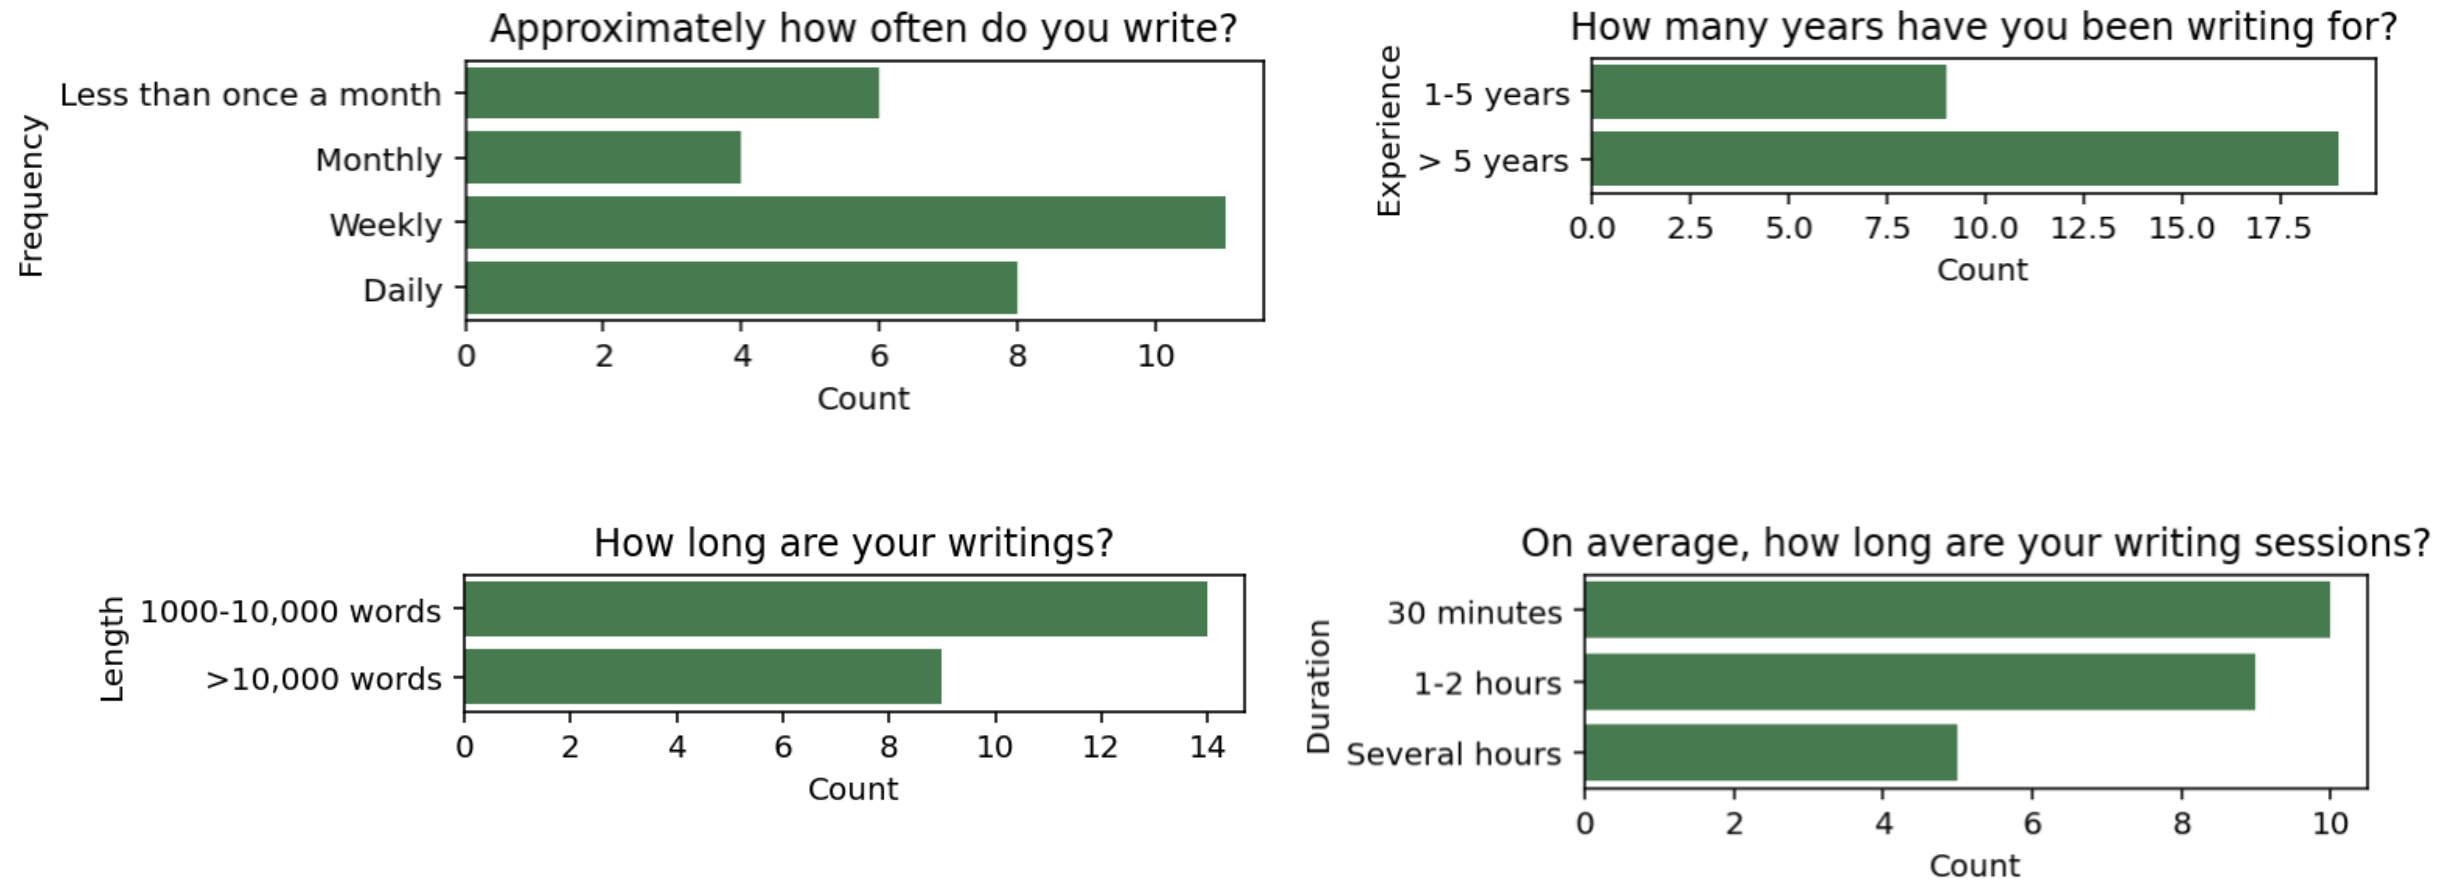
\includegraphics[width=\linewidth]{figures/recruitment_survey.png}
  \caption{Writing habits survey results.}
  \label{fig:writing_habits}
\end{figure}

\noindent We recruited participants via advertisements on Google-internal mailing lists. We then screened for individuals who practice creative writing on a regular basis, but who had not yet published their writing. 
Participants volunteered for the study and were not compensated. 
Most of the participants (23 out of 25) did not consider themselves to be machine learning practitioners and had not interacted with a generative language model previously.
We asked participants to complete a pre-study questionnaire about their writing habits (Figure \ref{fig:writing_habits}).
Then we carried out a within-subjects study, giving each user three writing prompts and asking them to write 100-300 word stories under the following three experimental conditions (illustrated in Figure \ref{fig:conditions}):

\begin{enumerate}
    \item \textbf{full} Wordcraft, as described in Section \ref{sec:wordcraft}.
    \item \textbf{cont} (baseline) a text editor with a single control: LaMDA will propose continuations to the text written so far. The \textit{cont} condition enables us to evaluate Wordcraft against existing AI-assisted writing applications which most often feature continuation as a single control.
    \item \textbf{chat} (baseline) a plain text editor shown alongside a chat dialog window.
    Users can converse with the LaMDA-powered chatbot, but the chatbot only ``knows'' what the user types to it.
    The \textit{chat} condition enables us to evaluate the utility of the prompt and UX scaffolding we designed for Wordcraft against giving users straightforward access to the underlying model, without any scaffolding. An omniscient user could theoretically reproduce the functionality of the \textit{full} condition by replicating Wordcraft's prompts.
\end{enumerate}

\begin{figure*}[t]
  \centering
  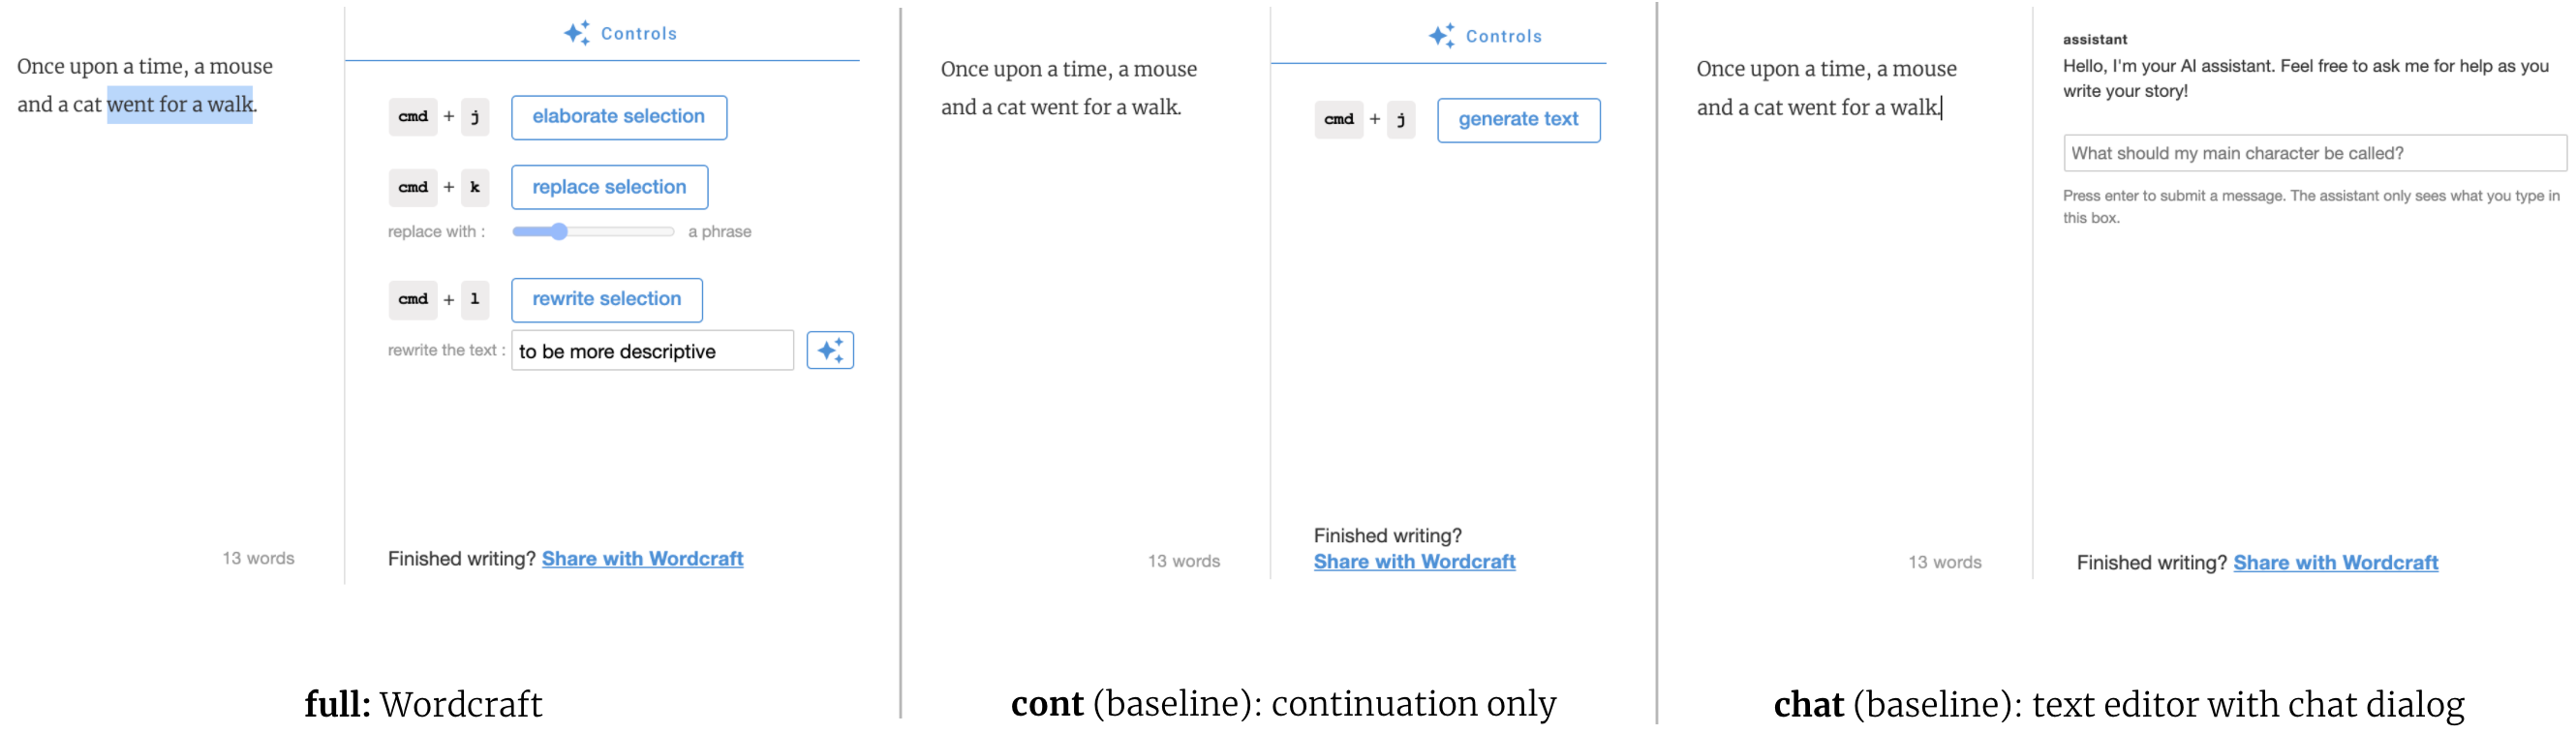
\includegraphics[width=1\linewidth]{figures/conditions.png}
  \caption{Experimental conditions for the user study. The stories written by participants as part of the study can be viewed here: \href{https://storage.googleapis.com/wordcraft-stories/index.html}{https://storage.googleapis.com/wordcraft-stories/index.html}. The website also includes purely machine-generated baselines.}
  \label{fig:conditions}
\end{figure*}

\noindent Participants were asked to write stories based on the following three prompts \footnote{Prompts were selected from the \href{https://www.reddit.com/r/WritingPrompts/}{Writing Prompts subreddit}.}:
\begin{enumerate}
    \item You arrive at Grandma's funeral to find thousands of people from around the world also in mourning. You are entirely unaware that Grandma had 16.4m followers on Twitter.
    \item All of the `No. 1 Dad' mugs in the world change to show the actual ranking of Dads suddenly.
    \item You lost your sight - along with everyone else on Earth - in The Great Blinding. Two years later, without warning, your sight returns. As you look around, you realize that every available wall, floor and surface has been painted with the same message - Don't Tell Them You Can See.
\end{enumerate}

\noindent Participants were given ten minutes to write each story.
We felt that ten minutes was enough time for users to acquaint themselves with the interface and write 100-300 words, while managing users' expectations for how much time they would need to spend on the study in total.
To control for writing ability and prompt difficulty, for each user, the three conditions were randomly paired with the three prompts, and the user was asked to write a story for each setting.
We also randomized the order in which the conditions were presented.
Users were not given any training for the various conditions``they were simply given a website link and asked to write a story with the interface.
Users were told that they were participating in a study of AI assisted writing, but they were not explicitly asked to solicit help from the AI agent, as we were interested in learning how often users would want to make use of AI-assisted controls.

\subsubsection{Results}
\label{sec:results}
This section describes the overall successes and failures of the NLG-powered assistive writing features incorporated into Wordcraft, before comparing Wordcraft to the baseline conditions in depth. 

\begin{table*}[t]
  \centering
  \caption{Usage statistics.}
  \small
  \label{tab:freq}
  \begin{tabular}{lllll}
    \toprule
    Property&\textit{chat} Chat&\textit{cont} Continuation&\textit{full} Wordcraft&Overall\\
    \midrule
    Requests made avg&6.3 \textpm 1.3&4.3 \textpm 0.52&7.3 \textpm 0.74&6.0 \textpm 0.53\\
    Accepted suggestions avg&N/A&0.17 \textpm 0.08&1.3 \textpm 0.25&0.51 \textpm 0.12\\
    Story word count avg&233 \textpm 18&237 \textpm 16 &267 \textpm 21.6&247 \textpm 11.1\\
    Model word count avg (\% of story)&N/A&2.9 \textpm 2 (1.3\%)&42.3 \textpm 14.2 (13.2\%)&16.2 \textpm 5.7 (5.2\%)\\
    Time considering suggestions avg&N/A&67.1s \textpm 8.7s&41s \textpm 4.1s&44.5s \textpm 3.2s\\
    Time to complete avg&11m \textpm 62.5s&11.52m \textpm 131.5s&9.97m \textpm 37.1s&10.8m \textpm 48.6s\\
  \bottomrule
\end{tabular}
\end{table*}

\begin{table}
  \caption{Usage statistics broken down by request type (Wordcraft only).}
  \small
  \label{tab:freq_wc}
  \begin{tabular}{lll}
    \toprule
    Request type&Requests made&Suggestions accepted\\
    \midrule
    Rewrite&27&5 (18.5\%)\\
    Story seed&22&12 (54.5\%)\\
    Suggest a prompt&40&2 (5\%)\\
    Fill-in-the-blank&4&0 (0\%)\\
    Continue&36&4 (11.1\%)\\
    Next sentence&7&1 (14.3\%)\\
    Elaborate&3&0 (0\%)\\
    Custom&51&9 (17.6\%)\\
  \bottomrule
\end{tabular}
\end{table}

\begin{table}
\caption{Rewrite requests (user completions of `Rewrite this...`)}
\label{tab:rewrites}
\small
% \resizebox{\columnwidth}{!}{%
% \def\arraystretch{1.5}% 
\begin{tabular}{p{1.0\columnwidth}}
\toprule
to be a little less angsty • to be about mining • to be better written • to be less diabolical • to be more absurd • to be more adventurous • to be more Dickensian • to be more emotional • to be more magical • to be more melodramatic • to be more philosophical • to be more revolutionary • to be more surprising • to be more suspenseful • to be more technical • to be more whimsical • to be warmer • to fit better grammatically with the rest of the story • to make more sense \\
\bottomrule
\end{tabular}
\end{table}

\begin{table}[t]
\caption{Custom prompts written by users.}
\label{tab:custom_prompts}
\small
\def\arraystretch{1.5}% 
\begin{tabular}{p{1.0\columnwidth}}
Tell me more about her twitter account.
• More about the dad please. • Tell me about Elaine's amazing twitter account. • Tell me about the father. • Tell me about the funeral home, grandma, the punk kid, and the crowd. • Tell me how the man reacted as he found out he could see again. • Tell me more about Daniel. • Tell me more about what it's like to have to pretend to be blind when you can see. • Tell me what happens next. • Tell me what the letter says. • What are the words on the floor? What language are they in? • What would happen if we could quantify love? • Why were they watching me? • More about the dad please. • So this guy was tight with your grandma? • Tell me about Elaine's amazing twitter account. • Tell me about the father. • Tell me about the funeral! • Tell me about the funeral home, grandma, the punk kid, and the crowd. • Tell me how the man reacted as he found out he could see again. • Tell me more about Daniel. • Tell me more about what it's like to have to pretend to be blind when you can see. • Tell me what happens next. • Tell me what the letter says. • What are the words on the floor? What language are they in? • What would happen if we could quantify love? • Who is telling me not to tell them? • Why were they watching me?
\end{tabular}
\end{table}

\subsection{The role of AI in co-writing}
\label{sec:results-idea-generator}

We observed that users solicited help from the AI agent at every stage of the writing process--from high-level story concepting down to rewriting and editing.
Thus, we found that the AI agent played many different roles in collaborative writing.

Users asked the AI agent for help in story ideation and brainstorming.
For example, nine users at one point presented the AI agent with their story and asked simply: \textit{`What happens next?'}.
Another user solicited help developing the premise for their story: \textit{`What would happen if we could quantify love?'}. 

Another typical use case for soliciting help from the AI was when just starting a story.
The story seed control, in which the AI agent provides opening sentences for a story given a writing prompt, had the highest success rate of any control: 55\% (Table \ref{tab:freq_wc}) of suggestions were accepted by users.
In these cases, the AI served to kick-start the writing process for users who might have been blocked.
Users also found the AI agent helpful for generating smaller scale details for their story, such as names for characters and locations.

Many users remarked on the usefulness of the AI agent's suggestions, even if they didn't end up using them verbatim: \textit{`Multiple suggestions around the highlight or next phrasing were very helpful, even if I didn't use the whole phrase ... it was like having someone suggest things that I might have thought of myself'} (U9).
Another user commented: \textit{`It was good at generating a bunch of relevant ideas that inspire my next lines and get me unstuck. I was never tempted to use any of the lines verbatim, but it was fun inspiration'} (U4).
Some also noted the AI agent's tendency to provide offbeat suggestions as a strength: \textit{`the off the wall suggestions were fun to play around with and helped shape how the story took form'} (U5).

We also observed users having ideas for events before knowing how they fit into an existing story - and in such cases asking the AI agent to fill in gaps.
For example, users would build a scene and then ask the AI agent to provide plot points that would contextualize the scene. 
One user in their story described a character being watched, and then asked the AI agent \textit{`Why were they watching me?'}. 
Many of the custom prompts (Table \ref{tab:custom_prompts}) we collected fall under this use case. 
These included prompts such as \textit{`Tell me what the letter says.'} and \textit{`Tell me about the funeral home, grandma, the punk kid, and the crowd.'}.

We also observed users asking the AI agent for help in smaller scale edits, for example: \textit{`Rewrite this sentence to fit better grammatically with the rest of the story'}, or \textit{`Rewrite this sentence to make more sense.'} 
Many of the requests in Table \ref{tab:rewrites} fall under this category. 

% \subsubsection{AI as search engine}
% We also found that in the \textit{chat} condition, users asked the AI for help in looking up information, such as \textit{'How many dads are there in the world?'}, or \textit{How do you cook pork chops?}. 

\subsubsection{Shortcomings of AI in co-writing}

The user study revealed many shortcoming in AI co-writing.
Users' observations of the AI agent's shortcomings mostly center on its lack of contextual awareness. 
For example, though the assistant might provide several fluent, well-written alternatives to a sentence as part of the rewrite control, its suggestions do not necessarily make sense given the rest of the story. One user whose story mentioned numbers moving on a coffee mug received suggestions from the AI agent which implied that \textit{`live animals (snakes specifically) were moving'}.
Users also noted many grammatical issues, for example that the AI agent's suggestions were often not in the same tense as the rest of the story. Some also noted that the AI did not seem aware of their story's established point of view (first person versus third person). 

% Quotes:
% \begin{itemize}
%     \item Understanding context - I was talking about the numbers on the mug constantly moving. But, the prompt/suggestions seemed to suggest that it was live animals (snakes specifically) that was moving.
%     \item More contextual awareness
%     \item AI does not seem to understand the direction of the story at more than a sentence level.
% \end{itemize}


% Quotes:
% \begin{itemize}
%     \item It used third person when I was writing in 1st person.
%     \item some of the suggested texts were in a different tense / viewpoint than my story
% \end{itemize}

\subsubsection{Wordcraft versus baseline 1: continuation-only}
In this section we compare Wordcraft to the continuation-only baseline (\textit{cont}). 
This baseline allows us to measure the utility of Wordcraft's prompting methods (Section \ref{sec:novel_prompt}) and UX patterns (Section \ref{sec:ux_patterns}) for the story writing task against the typical experience of \textit{continue-my-text} seen in existing LLM-powered writing tools.
We analyzed the activity logs from each user's writing session, and extract quantitative findings based on the following metrics (results in Table \ref{tab:freq}):

\begin{itemize}
    \item \textit{Requests made avg}: On average, how many times the user requested assistance from the AI while writing a story.
    \item \textit{Accepted suggestions avg}: On average, how many of the AI's suggestions the user accepted.
    \item \textit{Time considering suggestions avg}: The average time users spent between soliciting help from the AI, and accepting a suggestion or dismissing the suggestions.
    \item \textit{Model word count avg}: The average number of words in the final story that came directly from the AI agent.
    \item \textit{Time to complete avg}: The average time spent to produce the final story.
\end{itemize}

% \subsubsection{Users solicited and accepted more assistance from the AI using Wordcraft.}

Participants made significantly more requests of the AI agent using Wordcraft (7.31 \textpm 0.74) than the continuation-only baseline (4.35 \textpm 0.52) according to a paired-sample T-test (\textit{p} = 0.003). Participants also \textit{accepted} significantly (\textit{p} = 0.0003) more of the AI's suggestions using Wordcraft (1.27 \textpm 0.25 vs 0.17 \textpm 0.079). Accordingly, the stories written with Wordcraft contained significantly (\textit{p} = 0.0068) more text from the AI agent (13.2\% \textpm 3.8\%) than stories written with continuation-only (1.3\% \textpm 0.92\%).

% \subsubsection{Users spent less time to write longer stories using Wordcraft.}

% Users spent less time overall using Wordcraft (9.97m \textpm 37s) than continuation-only (11.52m \textpm 131.5s), even though the stories they wrote with Wordcraft are longer (267.7w \textpm 21.6w versus 237.3w \textpm 16w). However, these differences are not statistically significant.

% \subsubsection{Users found Wordcraft more helpful.}
The results from the Likert-scale questions in the exit interviews are in Figure \ref{fig:exit_interview_results}. According to a Mann-Whitney U test, users found Wordcraft significantly more helpful than the continuation-only baseline (\textit{p} = 0.0266).

% \subsubsection{Users enjoyed using controls aside from continuation.}
% \label{sec:extra_continuation}
We found that participants enjoyed using controls aside from continuation.
We note in Figure \ref{fig:favorite_ops} that more than half of the responses to the question `Which controls did you enjoy using' indicate controls \textit{other} than `generate text' (aka continuation). `Use your own prompt' was the most used control and the second most highly voted control, suggesting users enjoyed having the ability to design their own prompts. Table \ref{tab:freq_wc} lists the number of times each control was used and accepted in Wordcraft, further demonstrating that participants found utility in a variety of controls other than continuation. 

\subsubsection{Wordcraft versus baseline 2: chat}
In this section we compare Wordcraft to the \textit{chat} baseline. 
This again allows us to measure the importance of Wordcraft's prompting methods and UX patterns, but also to observe how writers might make use of a powerful open-domain LLM-powered chatbot in their creative process.
As the two conditions present significantly different user experiences, many of the metrics from the previous section are not applicable.
Thus we also analyze the chat transcripts and free-response exit interview questions to extract qualitative themes.

According to a Mann-Whitney U test, users found Wordcraft significantly more helpful than the chat baseline (\textit{p} = 0.0134), and also found it to be significantly more collaborative (\textit{p} = 0.00668).  
Nevertheless, we observed high user engagement with the chatbot assistant - on average users sent 6.3 \textpm 1.3 messages to the chatbot (Table \ref{tab:freq}). One user remarked: \textit{The AI agent asked good probing questions that gave me inspiration} (U22). Many talked to the chatbot the way a writer might discuss a project with a friend, asking for suggestions about overall direction as well as story details. For example (U1):


% \subsubsection{Users spent less time to write longer stories using Wordcraft.}

% Users spent less time overall using Wordcraft (9.97m \textpm 37s) than chat (11m \textpm 62s), even though the stories they wrote with Wordcraft are longer (267.7w \textpm 21.6w versus 232w \textpm 18w). However, these differences are not statistically significant.


\begin{quote}
    {\color{blue}\textit{user}:} How should I start a story about being blind?\\
    {\color{blue}\textit{AI agent}:} It's a unique perspective, so focus on description. What can you hear, smell, taste, and touch? These should all be used in your story.
\end{quote}

\noindent Another user (U4) asked about specific plot elements and character details:

\begin{quote}
    {\color{blue}\textit{user}:} what is grandma famous for on twitter?\\
    {\color{blue}\textit{AI agent}:} She is known on Twitter for her love for cooking with the great recipe ideas she shares and her love for gardening and giving advice for what you can grow in yours.\\
    {\color{blue}\textit{user}:} what cake recipe is grandma famous for\\
    {\color{blue}\textit{AI agent}:} She is known for her classic Victoria sponge cake recipe. Her recipe has over 5,000 likes which makes it one of her most popular.\\
    {\color{blue}\textit{user}:} what is grandma's twitter handle\\
    {\color{blue}\textit{AI agent}:} Her twitter handle is @mylovelygrandma where she regularly tweets her cooking tips and photos of her bountiful garden.
\end{quote}

Finally, participants found the chatbot to be effective at retrieving information. Some treated the chatbot as a search box, asking questions such as: \textit{how many people are fathers around the world}. In the exit interview, one user commented about the chatbot: ''\textit{I loved that it felt like a more targeted version of Google, and I could do background research while writing}'' (U21).

\subsection{User Study with Expert Writers}

\TODO{Write this section}
